% arara: pdflatex: { shell: yes }
% arara: biber
% arara: pdflatex
% arara: pdflatex
%

\pdfminorversion=7  % see https://www.overleaf.com/learn/latex/%5Cpdfminorversion and https://www.overleaf.com/learn/latex/%5Cpdfinclusionerrorlevel
                    % and the answer in https://tex.stackexchange.com/questions/542343/epstopdf-pdfminorversion-7-error


\documentclass[a4paper, 12pt, oneside]{book}


%-----------------------------------------------------------------------------
% Packages
%-----------------------------------------------------------------------------
\usepackage[T1]{fontenc}            % Font encoding
\usepackage[utf8]{inputenc}         % Input encoding
\usepackage[english,italian]{babel} % Text Language (secondaria, primaria)
\usepackage[babel]{csquotes}        % Dipendenza di babel
\usepackage{microtype}              % Improves text writing
\usepackage[backend=biber,autolang=hyphen]{biblatex}% Imports biblatex package
\setcounter{biburlnumpenalty}{9000}
\setcounter{biburlucpenalty}{9000}
\setcounter{biburllcpenalty}{9000}
\addbibresource{BackMatter/Tesi.bib}% Import the bibliography file
\usepackage{standalone}
\usepackage{graphicx}               % Required for inserting images
\graphicspath{ {./Images/} }        % Folder path to images. Path relative to the main .tex file  
\usepackage{subfig}
\usepackage{caption}
\captionsetup{format=hang,labelfont=bf}
\usepackage{float}                  % For figures
\usepackage[x11names]{xcolor}
\usepackage{fancyhdr}               % For the headings      
\usepackage{listings}               % Uso dei listing per il codice
\usepackage{svg}
\usepackage{lipsum}                 % Dummy package
\usepackage{afterpage}
\usepackage[most]{tcolorbox}
\tcbuselibrary{breakable}
\usepackage{tikz}
\usetikzlibrary{mindmap,shadows}
\usepackage{shapepar}
\usepackage{titlesec}
\usepackage{comment}
\usepackage[font={itshape,small}]{quoting}
%\quotingsetup{font=small}
\usepackage{mathtools} % loads also amsmath package
\usepackage{amssymb}
\usepackage{amsfonts} % for \mathbb
\usepackage{amsthm}
\usepackage{bm}  % for accessing bold math symbols
\usepackage{cancel}
\usepackage{booktabs} % for tables
\usepackage{algorithm}
\usepackage{algpseudocode}  %load automatically the algorithmicx package
\usepackage{customization} % IMport custom preamble 
\usepackage[hidelinks]{hyperref}
\hypersetup{
    pdfstartview = XYZ null null 1.00,  % open the generated pdf with 100% zoom by default
    pdftitle={Tesi}, 
}

\captionsetup[algorithm]{name=Algoritmo}




%-----------------------------------------------------------------------------
% Document Start
%-----------------------------------------------------------------------------
\begin{document}



%-------------------------------------------------------------------------
\frontmatter
%-------------------------------------------------------------------------
%\begin{titlepage}

\thispagestyle{empty}

\begin{center}
    \Large{UNIVERSITÀ DEGLI STUDI DI \\ CASSINO E DEL LAZIO MERIDIONALE}
\end{center}

%---------------------
% Unicas_Emblem 
%---------------------
\begin{figure}[!htp]
    \centering
    \includegraphics[keepaspectratio=true,scale=0.25]{Images/Frontespizio/Unicas_logo.pdf}
\end{figure}

\begin{center}
    \normalsize{DIPARTIMENTO DI INGEGNERIA ELETTRICA \\ E DELL'INFORMAZIONE “MAURIZIO SCARANO”}
    \vspace{4mm}
    \\ \normalsize{CORSO DI LAUREA IN INGEGNERIA INFORMATICA \\ E DELLE TELECOMUNICAZIONI}
\end{center}


\vspace{7mm}


\begin{center}
    \LARGE{\textbf{Generatori di immagini \\ da prompt testuali: stato dell'arte}}
\end{center}


\vspace{20mm}


\begin{minipage}[t]{0.47\textwidth}
	{\normalsize{\textbf{Relatore:}}{\normalsize\vspace{3mm}
	\\ \large{Prof. Alessandro Bria}}}
\end{minipage}
\hfill
\begin{minipage}[t]{0.47\textwidth}\raggedleft
	{\normalsize{\textbf{Candidato:}}{\normalsize\vspace{3mm} 
        \\ \large{Giuseppe Alfieri}}}
\end{minipage}


\vspace{30mm}


{\centering{\large{ANNO ACCADEMICO 2022/2023}}\par}



%\end{titlepage}

\cleardoublepage
    \thispagestyle{empty}
        \vspace*{\stretch{1}}
            \begin{flushright}
                \textit{Alla cara memoria di mio padre Donato} \\ \vspace{5mm}
                         Se hai qualcuno nel cuore, \\
                         l'hai vicino per sempre. \\ \vspace{1.5mm}
                        \footnotesize Marcia Grad Powers, \textit{La principessa \\ che credeva nelle favole} \\ \vspace{5mm}
                        \normalsize “Credi che le persone scomparse che abbiamo amato ci lascino mai del tutto? Non credi 
                        che le ricordiamo più chiaramente che mai nei momenti di grande difficoltà? Tuo padre è vivo in te, Harry, e 
                        si mostra soprattutto quando hai bisogno di lui. [...] Quindi ieri notte hai visto tuo padre, Harry... 
                        l'hai trovato dentro di te.”\\ \vspace{1.5mm}
                \footnotesize J.K. Rowling, \textit{Harry Potter \\ e il prigioniero di Azkaban}
            \end{flushright}
        \vspace{\stretch{2}}
\cleardoublepage
% \newpage\shipout\null
\afterpage{\null\thispagestyle{empty}\clearpage}

\begingroup 
\titleformat{\chapter}
{\normalfont\Huge\bfseries\centering} %shape
%{\centering} % format
{}% label
{} % sep
{}  

\chapter*{Abstract}


I generatori di immagini da prompt testuali, quali \emph{Midjourney}~\cite{Midjourney}, sono in grado di creare, partendo da descrizioni testuali, 
immagini di alta qualità che siano quanto più fedeli possibile alla \emph{semantica} del testo. 
Queste tecnologie si avvalgono di modelli generativi che, a loro volta, sottendono l'impiego di reti neurali.

In questa tesi si fornirà, preliminarmente, una panoramica generale 
della modellazione generativa, declinata al contesto della generazione di immagini, 
congiuntamente ad una visione d'insieme delle famiglie di modelli generativi più in auge in letteratura.

Successivamente verrà discussa la \emph{ratio} sottesa a una delle tecnologie, nella pletora di modelli generativi, che 
rendono possibile la “magia” di generare immagini: i modelli probabilistici di diffusione del rumore (\emph{Denoising Diffusion Probabilistic Models}) (DDPM).


\endgroup
%\addcontentsline{toc}{chapter}{\numberline{}Abstract} % This will add a chapter-level (chapter) entry to the table of contents (toc) without a chapter number (\numberline{})

\tableofcontents % Prints the main table of contents



%-------------------------------------------------------------------------
%-------------------------------------------------------------------------
\mainmatter
%-------------------------------------------------------------------------
%-------------------------------------------------------------------------


%-------------------------------------------------------------------------
% Introduzione
%-------------------------------------------------------------------------
\chapter{Introduzione}



La generazione di immagini da prompt testuali è atta alla creazione di rappresentazioni visive realistiche e coerenti a partire da descrizioni linguistiche, 
avvalendosi di modelli generativi.

Stante la complessità che la generazione di immagini e la comprensione del testo \emph{eo ipso} rappresentano, 
la generazione di immagini da prompt testuali, essendo il combinato disposto delle due, presenta un'ulteriore difficoltà: 
il passaggio da un dominio di rappresentazione all'altro per convertire esplicite relazioni testuali tra entità, in immagini consistenti con il significato del testo. 

Inoltre, un buon modello deve poter mescolare concetti e stili che non ha mai visto prima per generare immagini inedite.
Ad esempio, non esistono ritratti di Kim Jong-Un in camera da letto che stringe degli orsacchiotti, 
ma, ricorrendo a tecnologie che sottendono l'addestramento di reti neurali, è possibile creare una siffatta immagine (Figura~\ref{fig:midjourney_figures}).
Inoltre, sarebbe auspicabile che il modello desumesse accuratamente il modo in cui gli oggetti nell'immagine generata si relazionano tra loro, 
in base alla semantica del messaggio testuale e \emph{come} viene conferito significato alle parole attraverso il contesto~\cite{fosterGenerativeDeepLearning2023}.
Ad esempio, l'immagine di “una persona con un salvagente che galleggia in mare” dovrebbe apparire molto dissimile da quella di 
“una persona con un salvagente in un mare di gente”. 

\smallskip
\noindent In questa trattazione si approfondirà la sola parte relativa alla generazione di immagini, piuttosto che il meccanismo 
con cui si estrapola la semantica da un blocco testuale e la conseguente creazione di un'immagine che ne rifletta il contenuto.

\noindent In particolare, il lavoro è così ripartito:
\begin{itemize}
\item nel \hyperref[chap:generative_modeling]{Capitolo 2} si chiarisce cosa si intenda per modellazione generativa e la si confronta con la modellazione discriminativa. Inoltre, si riporta una tassonomia di modelli generativi.
\item nel \hyperref[chap:diff_models]{Capitolo 3} si illustra dettagliatamente una particolare tipologia di modelli di diffusione, che ha rappresentato un contributo pionieristico nell'ambito della modellazione generativa:
i modelli probabilistici di diffusione del rumore (\emph{Denoising Diffusion Probabilistic Models}) (DDPM). Tali modelli rimuovono gradualmente il rumore 
da una versione corrotta di una data immagine, pervenendo, con l'ausilio di una rete neurale, ad una stima della distribuzione dell'immagine originale.
In appendice~\ref{appendix:probability_statistics} si riportano alcune nozioni di base di probabilità e statistisca a supporto della discussione dei suddetti modelli, 
mentre nelle appendici~\ref{appendix:details_loss} e~\ref{appendix:unet} se ne forniscono, rispettivamente, i dettagli matematici e architetturali.
\end{itemize}
 


\begin{figure}
    \centering
    \subfloat[][Prompt:\emph{“Pope Francis playing dj console, wearing dj headphones”}]
    {\includegraphics[width=.33\textwidth]{Pope_Francis}} \quad
    \subfloat[][Prompt:\emph{“Kim Jong-Un wearing hello kitty pattern pajama in bedroom holding a big hello kitty peluche”}]
    {\includegraphics[width=.33\textwidth]{Kim_Jong_Un}} \\
    \subfloat[][Prompt:\emph{“Trump escorted by police officers”}]
    {\includegraphics[width=.33\textwidth]{Trump}} \quad
    \subfloat[][Prompt:\emph{“Trump in prison doing bodybuilding”}]
    {\includegraphics[width=.33\textwidth]{Trump_in_prison_doing_bodybuilding}}
    \caption{Immagini da me create con \emph{Midjourney}~\cite{Midjourney}, corredate dai prompt testuali originali in lingua inglese.}
    \label{fig:midjourney_figures}
\end{figure}




%-------------------------------------------------------------------------
% Capitoli
%-------------------------------------------------------------------------
\chapter{La modellazione generativa}\label{chap:generative_modeling}




\section{Introduzione}

La modellazione generativa può essere definita come segue:
\begin{quoting}
        “La modellazione generativa è una branca del machine learning che prevede l'addestramento 
         di un modello per generare nuovi dati inediti, che sono correlati all'insieme di dati 
         di addestramento originale.”(David Foster, $2023$~\cite{fosterGenerativeDeepLearning2023})
\end{quoting}
    

\noindent Si consideri, ad esempio, un insieme di dati (\emph{dataset}) che annovera immagini di chitarre. È possibile \emph{addestrare} un modello generativo su tale dataset
per desumere le regole che governano le complesse relazioni sussistenti tra i pixel nelle immagini delle chitarre.
A valle della fase di addestramento, avvalendosi del suddetto modello, è possibile creare nuove immagini inedite di chitarre
che non erano presenti nel dataset di partenza (Figura~\ref{fig:gen_model}).



\begin{figure}
        \centering
        \includegraphics[keepaspectratio, scale=0.55]{Generative_model}
        \caption{Esempio di modello generativo. Fonte:~\cite{fosterGenerativeDeepLearning2023}.}
        \label{fig:gen_model}
\end{figure}



\noindent È importante osservare che un modello generativo è intrinsecamente \emph{probabilistico}. Infatti 
la peculiare capacità di un modello generativo di produrre dati inediti
sottende l'apprendimento della distribuzione incognita dei dati di addestramento, 
cosicché \emph{campionando} da tale distribuzione sia possibile generare nuove istanze di dati: ciò richiede una certa variabilità e incertezza.


Qualora il modello fosse scevro da qualsivoglia elemento di aleatorietà 
(e.g.\ il modello è semplicemente un calcolo fisso, come prendere il valore medio di ogni pixel nel set di dati,~\cite{fosterGenerativeDeepLearning2023}),
stante la sua natura deterministica, non sarebbe generativo.   

\section{Modellazione generativa e discriminativa a confronto} 



Per una più accurata comprensione della modellazione generativa si rende opportuno un confronto con la controparte: la \emph{modellazione discriminativa}.

In Figura~\ref{fig:discr_model} è riportato un modello discriminativo atto a 
discernere se la paternità di un dipinto è o no attribuibile a Van Gogh. 
\begin{figure}
    \centering
    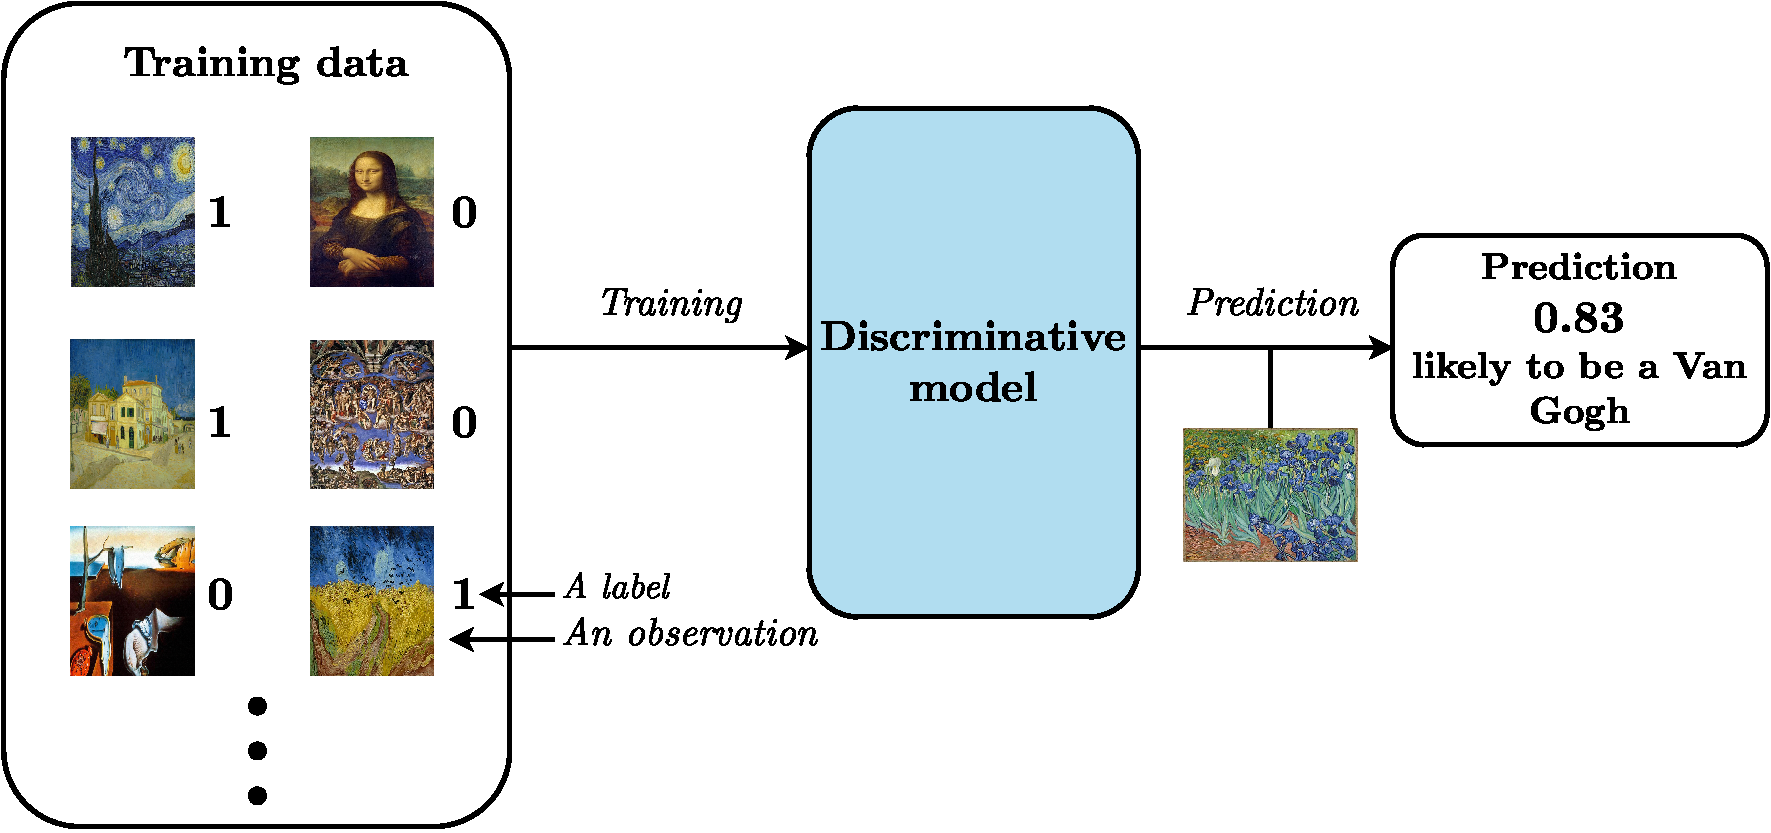
\includegraphics[keepaspectratio, scale=0.45]{Discriminative_model}
    \caption{Modello discriminativo addestrato a predire se una data immagine è stata dipinta da Van Gogh. Fonte:~\cite{fosterGenerativeDeepLearning2023}.}
    \label{fig:discr_model}
\end{figure}
Trattandosi di un tipico problema di classificazione binaria, il dataset di addestramento viene suddiviso in due gruppi:
i dipinti di Van Gogh vengono etichettati con $1$, laddove i dipinti di altri artisti sono etichettati con $0$. 
Il suddetto modello viene quindi addestrato a \emph{discriminare} tra i due gruppi e restituisce la probabilità 
che un'immagine, non presente nel dataset di addestramento, abbia come etichetta $1$(i.e.\ sia effettivamente un quadro di Van Gogh)~\cite{fosterGenerativeDeepLearning2023}.

\noindent Si noti come, nel contesto della modellazione discriminativa, ogni osservazione nel dataset di addestramento sia corredata da un'etichetta (\emph{label}).
Di converso, l'etichettatura del dataset di addestramento non costituisce un requisito essenziale nell'ambito della modellazione generativa, concernente la 
creazione di immagini inedite piuttosto che la corretta attribuzione dell'etichetta ad una data immagine.

\bigskip
\noindent Di seguito si formalizza matematicamente quanto appena esposto:
\begin{itemize}
\item i modelli discriminativi stimano la probabilità $p(y|\mathbf{x})$ che $y$ sia l'etichetta corrispondente ad una data osservazione $\mathbf{x}$ (Figura~\ref{fig:discr_model}).
\item i modelli generativi stimano la distribuzione incognita $p(\mathbf{x})$ dei dati del dataset di addestramento: il modello genera, quindi, nuovi dati a partire dalla distribuzione appresa.
\end{itemize}



\begin{oss}
Si noti che un modello generativo può anche stimare la probabilità condizionata $p(\mathbf{x}|y)$ di osservare il dato $\mathbf{x}$ la cui etichetta è $y$. 
Ad esempio, se il dataset di addestramento contenesse immagini di diversi tipi di alberi, si potrebbe ricorrere ad un modello generativo per generare un'immagine di un cipresso: in tal caso si parla di 
\emph{modelli generativi condizionati}~\cite{fosterGenerativeDeepLearning2023}.
\end{oss}


\noindent Dunque, mentre l'obiettivo della modellazione discriminativa è quello di classificare i dati in base alle loro caratteristiche (\emph{features}), 
la modellazione generativa concerne la creazione di nuovi dati che esibiscono affinità con il dataset di addestramento.




\section{Tassonomia dei modelli generativi}

Sebbene in questa trattazione si investigherà dettagliatamente solo una particolare categoria di modelli diffusione (i.e.\ i modelli di diffusione del rumore (DDPM)), 
è bene inquadrare il ruolo di quest'ultimi nel contesto più ampio dei modelli generativi che si avvalgono del metodo di massima verosimiglianza (Appendice~\ref{appendix:MLE}).
\begin{oss}
A rigore non tutti i modelli generativi ricorrono al metodo della massima verosimiglianza: le GAN, ad esempio, non utilizzano il metodo di massima verosimiglianza.
Tuttavia, “\emph{ignorando quei modelli che non ricorrono alla massima verosimiglianza, e concentrandosi sulla 
versione di massima verosimiglianza dei modelli che solitamente non utilizzano tale metodo (come le GAN), 
si possono eliminare alcune delle differenze che più distraggono tra
modelli diversi}”(Goodfellow, $2016$~\cite{goodfellowNIPS2016Tutorial2017}), a beneficio di una più compatta visione d'insieme dei modelli generativi.
\end{oss}
\begin{figure}
  \centering
  \includestandalone[mode=image,scale=0.8]{Images/tikz/gen_models_mindmap_rgb}
  \caption{Tassonomia dei modelli generativi. Adattato da~\cite{fosterGenerativeDeepLearning2023,goodfellowNIPS2016Tutorial2017}.}.
  \label{fig:gen_models_taxonomy}
\end{figure}
\noindent I modelli generativi che sottendono il ricorso al metodo della massima verosimiglianza (Appendice~\ref{appendix:MLE}) 
differiscono per il modo in cui rappresentano, o approssimano, la distribuzione di probabilità $p_{\bm{\theta}}(\mathbf{x})$\cite{goodfellowNIPS2016Tutorial2017}.

\noindent In letteratura si ravvisano tre approcci possibili~\cite{fosterGenerativeDeepLearning2023} nella modellazione di $p_{\bm{\theta}}(\mathbf{x})$:
\begin{itemize}
\item modellare \emph{esplicitamente} la suddetta distribuzione di probabilità.
\item modellare \emph{esplicitamente} un'\emph{approssimazione} della distribuzione di probabilità $p_\theta(\mathbf{x})$. 
\item modellare \emph{implicitamente} la distribuzione di probabilità $p_{\bm{\theta}}(\mathbf{x})$, delegando ad un processo stocastico la creazione dei dati.
\end{itemize}

\noindent In Figura~\ref{fig:gen_models_taxonomy} è riportata una \emph{tassonomia} dei modelli generativi.

\begin{oss}
Le famiglie di modelli riportate in Figura~\ref{fig:gen_models_taxonomy} non sono mutuamente esclusive: 
in letteratura si individuano molti esempi di modelli che sono degli ibridi tra approcci differenti.
Nella suddetta tassonomia, quindi, le diverse famiglie di modelli vanno interpretate come \emph{approcci generali} alla modellazione generativa, piuttosto 
che architetture esplicite di modelli~\cite{fosterGenerativeDeepLearning2023}.
\end{oss}

\noindent I modelli a densità implicita (\emph{Implict density models}) “non mirano a stimare la densità 
di probabilità $p_\theta(\mathbf{x})$, ma si concentrano unicamente sulla produzione di un processo stocastico 
che genera direttamente i dati”~\cite{fosterGenerativeDeepLearning2023}.

\medskip
\noindent I modelli a densità esplicita (\emph{Explicit density models}) si possono ulteriormente suddividere in quelli che ottimizzano direttamente 
la distribuzione di probabilità (\emph{tractable models}), e quelli che ottimizzano un'approssimazione della stessa.

\medskip
\noindent “\emph{Un filo conduttore che attraversa tutti i tipi di modelli generativi è il deep learning.
 Quasi tutti i modelli generativi più sofisticati sottendono il ricorso a reti neurali.}”~\cite{fosterGenerativeDeepLearning2023}.


\chapter{Modelli di diffusione}\label{chap:diff_models}

\section{Introduzione}

Scopo di questo capitolo è quello di analizzare la tecnologia che rappresenta il \emph{deus ex machina} del complesso processo 
che rende possibile la “magia” di generare immagini inedite da prompt testuali: i modelli di diffusione.

A rigore, nel contesto della generazione di immagini, i modelli di diffusione non sono l'unica opzione possibile nel panorama dei modelli generativi.
Tuttavia i modelli di diffusione, superando in termini prestazionali le GAN nella generazione di immagini (Dhariwal e Nichol, $2021$~\cite{dhariwal2021}),
sono assurti allo stato dell'arte in tale campo.

Il termine \emph{diffusione} è mutuato dal concetto di diffusione termodinamica: Sohl-Dickstein et al.\ ($2015$~\cite{sohl-dickstein2015}) 
hanno stabilito un importante collegamento tra tale concetto, inerente alla fisica, e il deep learning. 


Nel prosieguo si investigherà dettagliatamente la \emph{ratio} sottesa ad una particolare categoria di modelli di diffusione: 
i modelli probabilistici di diffusione del rumore (DDPM).

\section{Modelli probabilistici di diffusione del rumore (DDPM) }


I modelli probabilistici di diffusione del rumore (DDPM) sono stati introdotti in un articolo pubblicato nell'estate del 2020 (Ho et al.,~\cite{ho2020}) 
che ha segnato un punto di svolta nell'ambito dei modelli di diffusione e della modellazione generativa.

\medskip
\noindent La \emph{pipeline} di un DDPM è la seguente:
\begin{itemize}
\item nel \emph{processo di diffusione in avanti}, un'immagine è corrotta dal rumore fino a risultare, all'acme del processo, indistinguibile dallo stesso. 
La diffusione in avanti è funzionale a ricondursi, da un distribuzione di probabilità arbitrariamente complessa dell'immagine di partenza, al rumore puro che, invece, esibisce una distribuzione nota e 
facilmente manipolabile.
\item nel \emph{processo di diffusione inversa}, con l'ausilio di una rete neurale, si rimuove progressivamente il rumore, ripercorrendo a ritroso la diffusione in avanti, fino a pervenire all'immagine scevra da rumore. 
\end{itemize}


\subsection{Processo di diffusione in avanti}

Il processo di diffusione in avanti (\emph{forward diffusion process}) è definito come una \emph{catena markoviana} (si veda~\ref{ssec:markov_chain})
che va a perturbare la distribuzione originale, incognita, $q(\mathbf{x}_0)$ di un'immagine $\mathbf{x}_0$ del dataset di addestramento, 
corrompendola con rumore additivo gaussiano (Figura~\ref{fig:forward_diff_process}).

Qualora il suddetto rumore additivo abbia entità contenuta, le \emph{transizioni} della catena markoviana nel processo di diffusione in avanti possono essere 
modellate come distribuzioni gaussiane condizionate (Ho et al., $2020$~\cite{ho2020}). Avvalendosi del formalismo matematico risulta che:
\smallskip
\begin{Mybox1}
\begin{align}
  q(\mathbf{x}_{1:T}|\mathbf{x}_0)  & \triangleq \prod\limits_{t=1}^{T}q(\mathbf{x}_t|\mathbf{x}_{t-1})\quad\quad \text{Processo di diffusione in avanti} \label{eq:forward_process}\\
  q(\mathbf{x}_t | \mathbf{x}_{t-1}) & \triangleq \mathcal{N}(\mathbf{x}_t; \sqrt{1-\beta_t}\mathbf{x}_{t-1},\beta_t \bm{I}) \quad\quad  \text{Generica transizione}\label{eq:forward_chain_transition}
\end{align}
\end{Mybox1}
\smallskip
\noindent dove
\begin{itemize}
  \item $t\in[1,\dots,T]$ è il generico passo temporale.
  \item $\{\beta_t \in (0,1)\}_{t=1}^T$ implementano uno \hyperref[sssec:diff_schedules]{\emph{schema di diffusione}}.
  \item $\mathbf{x}_t$ è l'immagine a valle della $t$-esima transizione della diffusione in avanti.
  \item $\mathbf{x}_0$ è l'immagine originale di partenza che, dopo $T$ passi,
  converge a $\mathbf{x}_T$.
\end{itemize}
\bigskip
\noindent La~\eqref{eq:forward_chain_transition}, in virtù dell'\emph{artificio di riparametrizzazione} 
(si veda~\eqref{eq:rep_trick}), è equivalente ad asserire che
\begin{equation}\label{eq:rep_chain_transition}
 \mathbf{x}_t = \sqrt{1-\beta_t}\mathbf{x}_{t-1} + \sqrt{\beta_t}\bm{\epsilon}_{t-1} 
\end{equation}
dove $\bm{\epsilon}_{t-1} \sim \mathcal{N}(\mathbf{0},\bm{I})$.
\begin{oss}
  Si osserva esplicitamente che, nella~\eqref{eq:forward_chain_transition}, $\mathbf{x}_{t-1}$ è \emph{fissato}:
  il vettore  $\sqrt{1-\beta_t}\mathbf{x}_{t-1}$ è, quindi, \emph{deterministico}.
  Pertanto, dalla~\eqref{eq:forward_chain_transition} si evince che l'immagine $\mathbf{x}_t$ è distribuita come 
  una gaussiana condizionata con media $\bm{\mu}_t=\sqrt{1-\beta_t}\mathbf{x}_{t-1}$ e varianza $\bm{\Sigma}_t=\beta_t\bm{I}$.
\end{oss}
\medskip
\noindent Dalla~\eqref{eq:rep_chain_transition} si desume \emph{come} si ottiene l'immagine al passo 
temporale corrente $\mathbf{x}_t$ a partire dall'immagine $\mathbf{x}_{t-1}$ allo stato
precedente: ad una versione scalata di quest'ultima si aggiunge rumore gaussiano scalato.
Avendo l'accortezza di scegliere i $\beta_t$ opportunamente, si perverrà ad un'immagine $\mathbf{x}_T$ che, per $T$ sufficientemente elevato, 
approssima una distribuzione gaussiana standard ed è, pertanto, indistinguibile dal rumore gaussiano puro~\cite{ho2020}.
\begin{figure}
  \centering
  \includegraphics[keepaspectratio]{forward_process2456.pdf} 
  \caption{Processo di diffusione in avanti. Fonte~\cite{ho2020}.} \label{fig:forward_diff_process}
\end{figure}
\medskip
\begin{oss}
Il passaggio dalla~\eqref{eq:forward_chain_transition} alla~\eqref{eq:rep_chain_transition}, ricorrendo all'artificio di 
riparametrizzazione, sarà un \emph{pattern} ricorrente nel prosieguo, in particolare nella riformulazione del processo di diffusione in avanti 
atta a pervenire ad una versione ottimizzata dello stesso.
\end{oss}
\begin{oss}
  Il numero totale degli step di diffusione $T$ è un \emph{iperparametro} e, in quanto tale, 
  va fissato a monte della fase di addestramento del modello. Ho et al.\ ($2020$~\cite{ho2020}) hanno 
  propeso per $T=1000$. 
\end{oss}
\begin{oss}
  È importante osservare che, poiché ad ogni transizione della catena markoviana in avanti viene aggiunto solo del rumore, il
  processo di diffusione in avanti risulta \emph{fissato} qualora si scelgano i $\beta_t$.
\end{oss}
\medskip
\noindent Ricapitolando, il processo di diffusione in avanti trasforma, mediante l'aggiunta progressiva di rumore gaussiano, 
la complessa distribuzione incognita $q(\mathbf{x}_0)$ iniziale in una distribuzione normale standardizzata $\mathcal{N}(\bm{0},\bm{I})$. Il punto 
di forza di una siffatta distribuzione è insito nel suo essere facilmente manipolabile.
La distribuzione terminale della diffusione in avanti costituisce il punto di partenza del processo di diffusione inversa.



\subsubsection{Implementazione del processo di diffusione in avanti}

A beneficio di una maggiore ricchezza argomentativa, nonché per avere un riscontro pratico di 
quanto esposto precedentemente, viene riportata una possibile implementazione del processo di 
diffusione in avanti, partendo da una mia fotografia.

\begin{lstlisting}[language=iPython, caption=Codice adattato da~\cite{nain2022} e implementato con Google Colab~\cite{GoogleColaboratory},label=lst:diff]
import numpy as np                   # per manipolare array e matrici 
from PIL import Image                # per manipolare le immagini  
from matplotlib import pyplot as plt # per creare e visualizzare grafici 
from google.colab import files       # per scaricare l'immagine finale
  
def forward_diff_process(img_t_meno_(*@\color{black}{1}@*), beta, t):
    """
    Tale funzione implementa la generica transizione dall'immagine
    al passo t-1 all'immagine al passo t del processo di diffusione
    in avanti.

    Input:
        img_t_meno_1: immagine al passo precedente (*@$\mathcolor{ipython_red}{(\mathbf{x}_{t-1})}$@*)
        beta: schema di diffusione (vettore di numeri)
        t: passo corrente 
    Output:
        img_t: immagine a valle della transizione (*@$\mathcolor{ipython_red}{(\mathbf{x}_t)}$@*)
    """

    # 1. Si ricava (*@$\mathcolor{ipython_green}{\beta_t}$@*)
    beta_t = beta[t].reshape(-1, 1, 1)  

    # 2. Calcolo media statistica e deviazione standard
    mu = np.sqrt((1.0 - beta_t)) * img_t_meno_(*@\color{black}{1}@*)
    sigma = np.sqrt(beta_t)

    # 3. Generazione dell'immagine al passo t tramite l'equazione(*@\color{ipython_green}{~\eqref{eq:rep_chain_transition}}@*)
    img_t = mu + sigma*np.random.randn(*img_t_meno_(*@\color{black}{1}@*).shape)
    return img_t  

# ------------------------------------------------------------
# Esempio di applicazione del processo di diffusione in avanti  
# ------------------------------------------------------------

# 1. Si carica l'immagine di partenza (*@\color{ipython_green}{$\mathbf{x}_0$}@*)
img = Image.open("../content/selfie.jpg")

# 2. Si ridimensiona l'immagine secondo le dimensioni desiderate
IMG_SIZE = (100, 172)
img = img.resize(size=IMG_SIZE)

# 3. Si definisce il numero dei passi temporali (T)
timesteps = 100

# 4. Implementazione schema di diffusione lineare
beta_start = 0.0001
beta_end = 0.05
beta = np.linspace(beta_start, beta_end, num=timesteps, dtype=np.float(*@\color{black}{32}@*))

immagini_processate = [] 
img_t = np.asarray(img.copy(), dtype=np.float(*@\color{black}{32}@*)) / 255.

# 5.  Esecuzione del processo di diffusione in avanti
#     per ottenere l'immagine a valle di (*@$\mathcolor{ipython_green}{T=100}$@*) passi
for t in range(timesteps):   (*@\label{line:fw_diff}@*)                                                                
    img_t = forward_diff_process(img_t_meno_(*@\color{black}{1}@*)=img_t, beta=beta, t=t)
    if t%20==0 or t==timesteps - 1:   
        immagine = (img_t.clip(0, 1) * 255.0).astype(np.uint(*@\color{black}{8}@*))
        immagini_processate.append(immagine) (*@\label{line:fw_diff1}@*)

# 6. Visualizzazione delle immagini per diversi passi di diffusione
_, ax = plt.subplots(1, len(immagini_processate), figsize=(15, 8))

for i, immagine in enumerate(immagini_processate):
    ax[i].imshow(immagine)
    ax[i].set_title((*@\color{blue}{f}@*)"Timestep: (*@\color{ipython_green}{\{}\color{black}{i}\color{ipython_purple}{*}\color{black}{20}\color{ipython_green}{\}}@*)",fontsize=18)
    ax[i].axis("off")
    ax[i].grid(False)

plt.suptitle("Processo di diffusione in avanti", fontsize=22, y=0.78)
plt.savefig("forward_diff.pdf",pad_inches=0,bbox_inches='tight')
files.download('forward_diff.pdf')
plt.show()
plt.close()
\end{lstlisting}
\smallskip
\begin{center}
\includegraphics[keepaspectratio, scale=0.4]{code_result.pdf}
\end{center}

\noindent Si noti la progressiva perdita di connotati dell'immagine di partenza che, a valle di 
$T$ passi di diffusione, risulta indistinguibile dal rumore puro. 


%--------------------------------------------------------------

\subsubsection{Ottimizzazione del processo di diffusione in avanti}


Da un'attenta analisi del codice~\ref{lst:diff}, in particolare dalla riga~\ref{line:fw_diff} alla riga~\ref{line:fw_diff1}, si evince 
che, per pervenire all'immagine terminale $\mathbf{x}_T$, è necessario simulare l'\emph{intera} catena markoviana della diffusione in avanti:
all'aumentare del numero di step totali $T$ ciò risulta fortemente inefficiente.
Per ovviare a tale problema, definendo preliminarmente
\begin{equation}
  \alpha_t \triangleq  1-\beta_t, \quad\quad \overline{\alpha}_t  \triangleq \prod\limits_{i=1}^{t}\alpha_i \label{eq:alphas}
\end{equation} 
Ho et al.~\cite{ho2020} hanno osservato che la~\eqref{eq:rep_chain_transition} ammette la seguente riformulazione:
\begin{align}
\mathbf{x}_t & = \sqrt{1-\beta_t}\mathbf{x}_{t-1}+\sqrt{\beta_t}\bm{\epsilon}_{t-1}  \label{eq:eff_forward1}   \\ 
             & = \sqrt{\alpha_t}\mathcolor{blue}{\mathbf{x}_{t-1}}+\sqrt{1-\alpha_t}\bm{\epsilon}_{t-1}  \label{eq:eff_forward2}   \\ 
             & = \sqrt{\alpha_t}\bigl(\mathcolor{blue}{\sqrt{\alpha_{t-1}}\mathbf{x}_{t-2}+\sqrt{1-\alpha_{t-1}}\bm{\epsilon}_{t-2}}\bigr) + \sqrt{1-\alpha_t}\bm{\epsilon}_{t-1} \label{eq:eff_forward3}\\
             & = \sqrt{\alpha_t\alpha_{t-1}}\mathbf{x}_{t-2}+\mathcolor{red}{\sqrt{\alpha_t(1-\alpha_{t-1})}\bm{\epsilon}_{t-2}+\sqrt{1-\alpha_t}\bm{\epsilon}_{t-1}} \label{eq:eff_forward4}\\ 
             & = \sqrt{\alpha_t\alpha_{t-1}}\mathbf{x}_{t-2} + \mathcolor{red}{\sqrt{1-\alpha_t\alpha_{t-1}}\overline{\bm{\epsilon}}_{t-2}} \label{eq:eff_forward5} \\
             & = \dots \\
             & = \sqrt{\alpha_t\alpha_{t-1}\dots\alpha_1}\mathbf{x}_0 + \sqrt{1-\alpha_t\alpha_{t-1}\dots\alpha_1}\bm{\epsilon}_0 \\
             & = \sqrt{\overline{\alpha}_t}\mathbf{x}_0+\sqrt{1-\overline{\alpha}_t}\bm{\epsilon}_0, \label{eq:eff_forward}  
\end{align}

\noindent dove:
\begin{itemize}
  \item $\{\overline{\bm{\epsilon}}_{t},\bm{\epsilon}_{t}\}_{t=0}^T\overset{\text{iid}}{\sim} \mathcal{N}(\bm{0},\bm{I})$.
  \item dalla~\eqref{eq:eff_forward2} alla~\eqref{eq:eff_forward3} ci si è avvalsi dell'artificio di 
        riparametrizzazione~\eqref{eq:rep_trick}.
  \item il passaggio dalla~\eqref{eq:eff_forward4} alla~\eqref{eq:eff_forward5} è il combinato disposto dell'artificio di riparametrizzazione e 
  del risultato per cui una combinazione lineare di vettori gaussiani 
  \emph{indipendenti} è ancora un vettore gaussiano~\eqref{eq:comblingauss_scalar}. Infatti, poiché
  \begin{align}
    \sqrt{1-\alpha_t}\bm{\epsilon_{t-1}} &\sim \mathcal{N}(\bm{0},(1-\alpha_t)\bm{I}) \label{eq:rep_trick1}\\
    \sqrt{\alpha_t(1-\alpha_{t-1})}\bm{\epsilon_{t-2}} &\sim \mathcal{N}(\bm{0},(\alpha_t-\alpha_t\alpha_{t-1})\bm{I}) \label{eq:rep_trick2}
  \end{align}
  ed essendo $\bm{\epsilon_{t-1}}$ ed $\bm{\epsilon_{t-2}}$ \emph{indipendenti}, la somma di~\eqref{eq:rep_trick1} e~\eqref{eq:rep_trick2} è distribuita come
  \[
    \mathcal{N}(\bm{0},(1-\alpha_t+\alpha_t-\alpha_t\alpha_{t-1})\bm{I})=\mathcal{N}(\bm{0},(1-\alpha_t\alpha_{t-1})\bm{I})
  \]
  il che, ricorrendo all'artificio di riparametrizzazione, equivale a:
  \[
    \sqrt{1-\alpha_t}\bm{\epsilon_{t-1}} + \sqrt{\alpha_t(1-\alpha_{t-1})}\bm{\epsilon_{t-2}}
    =\sqrt{1-\alpha_t\alpha_{t-1}}\overline{\bm{\epsilon}}_{t-2}
  \]
\end{itemize} 

\begin{figure}
  \centering
  \includegraphics[keepaspectratio, scale=0.8]{forward_process3.pdf}
  \caption{Passaggio diretto da $\mathbf{x}_0$ a $\mathbf{x}_t$. Fonte:~\cite{vaibhavsinghInDepthGuideDenoising2023}.}
 \label{fig:skip_steps}
\end{figure}

\noindent Pertanto, il processo di diffusione in avanti può essere così riformulato:
\begin{Mybox}
\begin{equation}
  q(\mathbf{x}_t|\mathbf{x}_0)=\mathcal{N}\bigl(\mathbf{x}_t;\sqrt{\overline{\alpha}_t}\mathbf{x}_0,(1-\overline{\alpha}_t)\bm{I}\bigr) \label{eq:forward_diff_v2}
\end{equation}
\end{Mybox}
\smallskip
\noindent La riformulazione~\eqref{eq:forward_diff_v2} del processo di diffusione in avanti, basata 
essenzialmente sull'applicazione ricorsiva dell'artificio di riparametrizzazione, apporta un duplice beneficio:
\begin{itemize}
\item dall'immagine di partenza $\mathbf{x}_0$ è possibile raggiungere un $\mathbf{x}_t$ \emph{qualsiasi} con un \emph{unico} step di diffusione in avanti (Figura~\ref{fig:skip_steps}).
\item per progettare uno \emph{schema di diffusione} è possibile avvalersi degli $\overline{\alpha}_t$, in luogo dei $\beta_t$ originali. Il vantaggio di ciò 
risiede nell'interpretazione di $\overline{\alpha}_t$ come la varianza del segnale (l'immagine di partenza $\mathbf{x}_0$) e 
$1-\overline{\alpha}_t$ come la varianza del rumore $\bm{\epsilon}$~\cite{fosterGenerativeDeepLearning2023}.
\end{itemize} 

\noindent Si riporta di seguito l'implementazione della versione ottimizzata del processo di diffusione in avanti, 
per corroborare la perfetta equivalenza sussistente tra le due formulazioni dello stesso, precedentemente investigate.


\begin{lstlisting}[language=iPython,caption=Diffusione in avanti ottimizzata. Codice adattato da~\cite{nain2022},label=lst:diff_ott]
import numpy as np                 
from PIL import Image             
from matplotlib   import pyplot as plt   
from google.colab import files     
    
def forward_diff_process_ott(img_orig, alpha_bar, t):
    """
    Input:
        img_orig: immagine al passo t=0 (*@$(\mathcolor{ipython_red}{\mathbf{x}_0})$@*)
        alpha_bar: versione riparametrizzata di beta
        t: passo corrente 
    Output:
        img_t: immagine ottenuta al passo corrente (*@$(\mathcolor{ipython_red}{\mathbf{x}_t})$@*)
    """
    
    # 1. Si ricava (*@$\mathcolor{ipython_green}{\overline{\alpha}_t}$@*)
    alpha_bar_t = alpha_bar[t].reshape(-1, 1, 1)
    
    # 2. Calcolo media statistica e deviazione standard
    mu = np.sqrt(alpha_bar_t) * img_orig
    sigma = np.sqrt(1.0 - alpha_bar_t)
    
    # 3. Generazione dell'immagine al passo t tramite l'equazione(*@\color{ipython_green}{~\eqref{eq:eff_forward}}@*)
    img_t = mu + sigma * np.random.randn(*img_orig.shape)
    return img_t
  

# 1. Si carica l'immagine di partenza (x0) 
img = Image.open("../content/selfie.jpg")
  
# 2. Si ridimensiona l'immagine secondo le dimensioni desiderate
IMG_SIZE = (100, 172)
img = img.resize(size=IMG_SIZE)
  
# 3. Si definisce il numero dei passi temporali (T)
timesteps = 100

#----------------------------------------------------------
# Versione ottimizzata del processo di diffusione in avanti  
#----------------------------------------------------------

# 4. Implementazione schema di diffusione lineare
beta_start = 0.0001
beta_end = 0.05
beta = np.linspace(beta_start, beta_end, num=timesteps, dtype=np.float32)

# 5. Si definiscono alpha e alpha_bar secondo la (*@\color{ipython_green}{\eqref{eq:alphas}}@*)
alpha = 1.0 - beta
alpha_bar = np.cumprod(alpha)
  
immagini_processate = [img] # immagine (*@$\mathcolor{ipython_green}{\mathbf{x}_0}$@*)
img_orig = np.asarray(img.copy(), dtype=np.float32) / 255.

# 6. Esecuzione del passo di diffusione in avanti per timestep specifici
# Si scelgono gli stessi timestep visualizzati nel codice (*@\color{ipython_green}{\ref{lst:diff}}@*)
timestep_specifici = [19, 39, 59, 79, 99]
for step in timestep_specifici:
    img_t = forward_diff_process_ott(img_orig, alpha_bar, step)
    img_t = (img_t.clip(0, 1) * 255.0).astype(np.uint8)
    immagini_processate.append(img_t)
  

# 7. Visualizzazione delle immagini in diversi passi di diffusione
_, ax = plt.subplots(1, len(immagini_processate), figsize=(15, 8))

for i, sample in enumerate(immagini_processate):
    ax[i].imshow(sample)
    ax[i].set_title((*@\color{blue}{f}@*)"Timestep: (*@\color{ipython_green}{\{}\color{black}{i}\color{ipython_purple}{*}\color{black}{20}\color{ipython_green}{\}}@*)",fontsize=18)
    ax[i].axis("off")
    ax[i].grid(False)

plt.suptitle("Diffusione in avanti ottimizzata",fontsize=22, y=0.78)
plt.savefig("forward_process_v2.pdf",pad_inches=0,bbox_inches='tight')
files.download('forward_process_v2.pdf')
plt.show()
plt.close()
\end{lstlisting}
\begin{center}
\includegraphics[keepaspectratio, scale=0.4]{efficient_forward_process.pdf}
\end{center}
Si noti che, sebbene il risultato del codice~\ref{lst:diff_ott} sia il medesimo del codice~\ref{lst:diff}, il discrimine tra i due è 
insito nel \emph{modo} in cui si perviene alle immagini nei diversi passi di diffusione.

%---------------------------------------------------------------------
\subsubsection{Schemi di diffusione}\label{sssec:diff_schedules}

\begin{figure}
  \centering
  \includegraphics[keepaspectratio, scale=0.9]{diff_schedules}
  \caption{Diversi schemi di diffusione. Fonte:~\cite{changDesignFundDiffusion2023}.}
  \label{fig:diff_schedules}
\end{figure}

Uno schema di diffusione si esplica in una particolare istanza del 
vettore\footnote{Abuso di notazione: l'apice $T$ è l'operazione di \emph{trasposizione},
il pedice $T$ è il numero totale degli step di diffusione.} $\bm{\beta}=(\beta_1,\dots,\beta_T)^T$, e controlla la quantità di rumore 
che viene aggiunta ad ogni passo della catena markoviana nel processo di diffusione in avanti.

\bigskip
\noindent In letteratura si ravvisano due approcci:
\begin{itemize}
\item si addestra una rete neurale ad apprendere i $\beta_t$ che, in tal caso, sono considerati alla stregua di 
parametri ordinari della rete.
Perseguendo tale approccio è possibile implementare schemi di diffusione \emph{diversi} per la fase di addestramento 
e la fase di inferenza~\cite{changDesignFundDiffusion2023}.
\item i $\beta_t$ assurgono ad iperparametri e, in quanto tali, sono fissati a priori (\emph{hyperparameter tuning}). In 
tal caso, per progettare i $\beta_t$, in letteratura, si ricorre ad un ampio ventaglio di tecniche \emph{euristiche}~\cite{changDesignFundDiffusion2023}.
\end{itemize}
Ho et al.~\cite{ho2020} hanno optato per quest'ultimo approccio, propendendo per uno schema di diffusione \emph{lineare} 
in cui i $\beta_t$ crescono linearmente da $\beta_1=10^{-4}$ a $\beta_T=0.02$.

Tuttavia, è stato dimostrato (Nichol et al., $2021$~\cite{nicholImprovedDenoisingDiffusion2021a}) 
che l'impiego di uno schema di diffusione sinusoidale implica un incremento delle prestazioni del modello di diffusione.
In Figura~\ref{fig:diff_schedules} sono riportati diversi schemi di diffusione.

Nel progettare uno schema di diffusione non si deve trascurare l'ingrediente fondamentale nel deep learning: i \emph{dati}.
Dal punto di vista della rappresentazione dei dati, la dimensionalità degli stessi e la massima distanza euclidea tra i campioni di addestramento 
sono fattori da contemplare nel design di uno schema di diffusione~\cite{songImprovedTechniquesTraining2020}. Inoltre, uno schema di diffusione deve 
tener conto della complessità e della ridondanza insita nei dati~\cite{chenImportanceNoiseScheduling2023}. Ad esempio, immagini più grandi potrebbero richiedere più 
rumore additivo, a parità di passi di diffusione in avanti, rispetto ad immagini di dimensioni più piccole~\cite{nicholImprovedDenoisingDiffusion2021a}.

Il \emph{tipo di rumore} aggiunto ad ogni passo del processo di diffusione in avanti è un altro iperparametro: Ho et al.~\cite{ho2020} hanno propeso 
per rumore gaussiano $\bm{\epsilon}\sim\mathcal{N}(\bm{0},\bm{I})$. 


\subsection{Processo di diffusione inversa}


La magia dei modelli di diffusione avviene nel processo di diffusione inversa (\emph{reverse diffusion process}). 
La \emph{ratio} sottesa al processo di diffusione inversa è quella di rimuovere iterativamente rumore
(\emph{denoising}) dall'immagine $\mathbf{x}_T\sim\mathcal{N}(\bm{0},\bm{I})$ (a cui si perviene a valle del processo di diffusione in avanti),
per risalire alla distribuzione incognita dell'immagine di partenza $q(\mathbf{x}_0)$ (Figura~\ref{fig:reverse_diff_process}).
Tuttavia per assolvere a tale scopo, il processo di diffusione inversa non può servirsi della distribuzione a posteriori
$q(\mathbf{x}_{t-1}|\mathbf{x}_t)$. Infatti, ricorrendo alla legge di Bayes~\eqref{eq:Bayes}, risulta che
\begin{equation}
    q(\mathbf{x}_{t-1}|\mathbf{x}_t)=\frac{q(\mathbf{x}_{t}|\mathbf{x}_{t-1})q(\mathbf{x}_{t-1})}{q(\mathbf{x}_t)} \label{eq:reverse_transition}
\end{equation}
da cui si evince come l'intrattabilità di $q(\mathbf{x}_{t-1}|\mathbf{x}_t)$ sia imputabile alle distribuzioni marginali $q(\mathbf{x}_{t-1})$ e $q(\mathbf{x}_t)$ 
in quanto~\footnote{Risultato analogo sussite \emph{mutatis mutandis} per $q(\mathbf{x}_{t-1})$}:
\begin{align}
    q(\mathbf{x}_t) &= \int q(\mathbf{x}_0,\mathbf{x}_1,\dots,\mathbf{x}_t)\,d\mathbf{x}_0\,d\mathbf{x}_1\dots\,d\mathbf{x}_{t-1} \label{eq:marginalization_op} \\
                    &= \int q(\mathbf{x}_1,\dots,\mathbf{x}_t|\mathbf{x}_0)q(\mathbf{x}_0) \,d\mathbf{x}_0\,d\mathbf{x}_1\dots\,d\mathbf{x}_{t-1} \label{eq:marginal}
\end{align}
dove $q(\mathbf{x}_1,\dots,\mathbf{x}_t|\mathbf{x}_0)$ è la catena markoviana della diffusione in avanti definita dalla~\eqref{eq:forward_process}, 
e nella~\eqref{eq:marginalization_op} si è effettuata l'operazione di marginalizzazione~\eqref{eq:marginalizzazione}.

Dalla~\eqref{eq:marginal} si evince chiaramente che il problema sotteso al calcolo di $q(\mathbf{x}_t)$ è duplice:
\begin{itemize}
\item la distribuzione $q(\mathbf{x}_0)$ è \emph{incognita}.
\item l'integrale nella~\eqref{eq:marginal}, essendo esteso ad uno spazio (di pixel) ad alta dimensionalità, è \emph{intrattabile}.
\end{itemize}
\begin{figure}
    \centering
    \includegraphics[keepaspectratio]{reverse_diff_process}
    \caption{Processo di diffusione inversa. Fonte:~\cite{ho2020}.}
    \label{fig:reverse_diff_process}
\end{figure}
Ho et al.~\cite{ho2020}, sulla scia di Sohl-Dickstein et al.~\cite{sohl-dickstein2015}, propongono l'addestramento di una rete neurale
per approssimare $q(\mathbf{x}_{t-1}|\mathbf{x}_t)$.

\noindent Il processo di diffusione inversa, quindi, è definito come un catena markoviana di transizioni gaussiane i cui parametri
(i.e.\ media e varianza) sono appresi 
da una rete neurale. L'assunzione di gaussianità per le suddette transizioni è supportata 
dall'osservazione che, qualora i $\beta_t$ abbiano entità contenuta, le transizioni di entrambi i processi 
di diffusione (diretta e inversa) esibiscono la stessa forma funzionale~\cite{fellerTheoryStochasticProcesses1949}.
Matematicamente risulta che:
\noindent 
\begin{Mybox1}
\begin{gather}
    p_{\bm{\theta}}(\mathbf{x}_{0:T})   \triangleq p(\mathbf{x}_T)\prod\limits_{t=1}^{T}p_{\bm{\theta}}(\mathbf{x}_{t-1}|\mathbf{x}_t) \, \text{Processo di diffusione inversa} \label{eq:reverse_process} \\
    p_{\bm{\theta}}(\mathbf{x}_{t-1}|\mathbf{x}_t) \triangleq \mathcal{N}(\mathbf{x}_{t-1}; \bm{\mu}_{\bm{\theta}}(\mathbf{x}_t,t),\bm{\Sigma}_{\bm{\theta}}(\mathbf{x}_t,t)) \,  \text{Generica transizione}\label{eq:chain_transition132}
\end{gather}
\end{Mybox1}
\noindent dove:
\begin{itemize}
\item $p(\mathbf{x}_T)=q(\mathbf{x}_T)=\mathcal{N}(\mathbf{x}_T;\bm{0},\bm{I})$ dal momento 
che il punto di arrivo della diffusione in avanti costituisce la base di partenza del processo di diffusione inversa.
\item il pedice $\bm{\theta}$ denota il vettore dei \emph{parametri} della rete neurale, aggiornati con la tecnica del gradiente discendente stocastico.
\item $\bm{\mu}_{\bm{\theta}}(\mathbf{x}_t,t)$,$\bm{\Sigma}_{\bm{\theta}}(\mathbf{x}_t,t)$ 
sono rispettivamente media e varianza che, come suggerisce la notazione (i.e il pedice $\bm{\theta}$), sono appresi dalla rete neurale.
\end{itemize}

\bigskip
\noindent Ricapitolando, il processo di diffusione inversa consiste nel rimuovere 
iterativamente (anziché in un singolo passo come le GAN~\cite{changDesignFundDiffusion2023}), servendosi di una rete neurale, 
il rumore dall'immagine $\mathbf{x}_T$. Tale processo di diffusione inversa è imbastito sull'immagine terminale della diffusione in avanti
e, al decrescere di $t$ da $T$ a $0$, si propaga nella direzione opposta a quest'ultima tramite una catena markoviana 
di transizioni~\eqref{eq:chain_transition132}.

\subsection{Addestramento}


Da quanto detto nel paragrafo precedente, \emph{si ricorre ad una rete neurale} 
per approssimare la media e la varianza delle transizioni~\eqref{eq:reverse_transition} intrattabili della diffusione inversa.


\noindent Nella scelta della funzione di costo da minimizzare per allenare la rete neurale, la \emph{ratio} perseguita è la seguente.
Dal momento che si possono ravvisare delle affinità tra il processo di diffusione inversa e il 
decoder di un \emph{autoencoder variazionale} (VAE) (si veda~\ref{fig:VAE_vs_Diff}), è 
legittimo avvalersi della medesima funzione di costo usata nei VAE: 
il logaritmo della funzione di verosimiglianza cambiato di segno (\emph{Negative Log-Likelihood})(\ref{ssec:verosimiglianza}).
Pertanto, la funzione di costo da minimizzare è:
\begin{equation}
 L=-\log\bigl(p_{\bm{\theta}}(\mathbf{x}_0)\bigr)
\end{equation}
Tuttavia, esplicitando la funzione di verosimiglianza $p_{\bm{\theta}}(\mathbf{x}_0)$
\begin{equation}
 p_{\bm{\theta}}(\mathbf{x}_0)=\int p_{\bm{\theta}}(\mathbf{x}_{0:T}) \,d\mathbf{x}_{1:T} \label{eq:intractable_likelihood}
\end{equation}
si desume che $p_{\bm{\theta}}(\mathbf{x}_0)$ (e quindi $L$) è \emph{intrattabile}, essendo 
l'integrale nella~\eqref{eq:intractable_likelihood} esteso ad uno spazio (di pixel) ad alta dimensionalità.
Si ricorre, quindi, al tipico \emph{pattern} di approssimare una funzione intrattabile con un suo \emph{lower bound} 
(Figura~\ref{fig:vlb}) che ammetta, invece, un'espressione in forma chiusa.
\begin{figure}
    \centering
    \includegraphics[keepaspectratio, scale=0.5]{lower_bound.pdf}
    \caption{\emph{Lower bound} di una funzione. Fonte~\cite{royBeginnerGuideDiffusion}.} 
    \label{fig:vlb}
\end{figure}
Invocando, ancora una volta, l'affinità intercorrente tra il processo di diffusione inversa e il decoder 
di un VAE, si può ricorrere al \emph{lower bound variazionale} (VLB) (o \emph{lower bound dell'evidenza} (ELBO)) che, 
declinato al contesto dei modelli di diffusione, è:
\begin{equation}
    \log \bigl(p_{\bm{\theta}}(\mathbf{x}_0)\bigr)\geq\underbrace{\mathbb{E}_q\biggl[\log\frac{p_{\bm{\theta}}(\mathbf{x}_{0:T})}{q(\mathbf{x}_{1:T}|\mathbf{x}_0)}\biggr]}_{VLB}
\end{equation}
(si veda Appendice~\ref{appendix:details_loss} per la derivazione dettagliata), e, come si vedrà nel prosieguo, risulterà essere trattabile. 
Pertanto, minimizzare la funzione di costo $L$ significa minimizzare il VLB cambiato di segno:
\begin{equation}
    L=-\log \bigl(p_{\bm{\theta}}(\mathbf{x}_0)\bigr)\leq L_{vlb}\triangleq\mathbb{E}_q\biggl[-\log\frac{p_{\bm{\theta}}(\mathbf{x}_{0:T})}{q(\mathbf{x}_{1:T}|\mathbf{x}_0)}\biggr]
\end{equation}
\begin{oss}
A rigore l'uso del pedice \emph{vlb} in $L_{vlb}$ è un abuso di notazione, dal momento che $L_{vlb}$ non è 
un lower bound ma è un \emph{upper bound} della funzione di costo $L$. Tuttavia, si predilige 
tale notazione $L_{vlb}$ per essere consistenti con la letteratura.
\end{oss}
\noindent A valle di una serie di calcoli che sono riportati in Appendice~\ref{appendix:details_loss} si perviene al seguente risultato:
\begin{equation}
    L_{vlb}=L_0+\sum_{t=2}^TL_{t-1}+L_T \label{eq:Lvlb}
\end{equation}
dove:
\begin{itemize}
    \item $L_0=-\log \bigl(p_{\bm{\theta}}(\mathbf{x}_0|\mathbf{x}_1)\bigr)$. Ho et al.~\cite{ho2020} hanno delegato ad un apposito decoder l'approssimazione di tale termine
    che, pertanto, può essere trascurato nella fase di addestramento della rete neurale.
    \item $L_{t-1}=D_{KL}\bigl(q(\mathbf{x}_{t-1}|\mathbf{x}_t,\mathbf{x}_0)\,\|\,p_{\bm{\theta}}(\mathbf{x}_{t-1}|\mathbf{x}_t)\bigr)$. L'obiettivo  
    è quello di addestrare la rete neurale, cosicché $p_{\bm{\theta}}(\mathbf{x}_{t-1}|\mathbf{x}_t)$ approssimi 
    quanto più fedelmente la distribuzione $q(\mathbf{x}_{t-1}|\mathbf{x}_t,\mathbf{x}_0)$ in 
    modo da minimizzare il termine $L_{t-1}$ (ricorrendo all'usuale interpretazione della \emph{divergenza di Kullback-Leibler} 
    (Appendice~\ref{appendix:details_loss},~\ref{eq:kullback-leibler})
    come una misura della distanza tra le distribuzioni).
    \item $L_T=D_{KL}\bigl(q(\mathbf{x}_T|\mathbf{x}_0)\,\|\,p(\mathbf{x}_T)\bigr)$ è un termine che può essere \emph{ignorato} durante 
    la fase di addestramento, dal momento che non annovera alcun parametro che possa essere appreso dalla rete neurale. 
    Infatti $p(\mathbf{x}_T)=q(\mathbf{x}_T)\sim\mathcal{N}(\bm{0},\bm{I})$ 
    e $q(\mathbf{x}_T|\mathbf{x}_0)$ è fissato una volta scelti gli iperparametri $\beta_t$~\eqref{eq:forward_diff_v2}.
\end{itemize}

\begin{oss}
    Definendo uno schema di diffusione opportuno (i.e.\ i valori dei $\beta_t$)
    e scegliendo l'iperparametro $T$ sufficientemente elevato, entrambe le distribuzioni 
    $q(\mathbf{x}_T|\mathbf{x}_0)$ e $p(\mathbf{x}_T)$ approssimano una gaussiana standard. 
    Quindi, stante l'interpretazione della divergenza di Kullback-Leibler come una misura della distanza tra tali distribuzioni,
    il termine $L_T=D_{KL}\bigl(q(\mathbf{x}_T|\mathbf{x}_0)\,\|\,p(\mathbf{x}_T)\bigr)$ tende a zero.
\end{oss}
\noindent Dunque, affinché $L_{vlb}$ risulti trattabile è sufficiente che $L_{t-1}$ ammetta un'espressione in forma chiusa.

\noindent Restringendo l'attenzione al termine $L_{t-1}$, 
in Appendice~\ref{sec:detailed_loss_term} si mostra che sussistono le seguenti considerazoni:
\begin{itemize}
\item poiché:
\begin{align}
    q(\mathbf{x}_{t-1}|\mathbf{x}_t,\mathbf{x}_0) &= \mathcal{N}(\mathbf{x}_{t-1}; \tilde{\bm{\mu}}_{t}(\mathbf{x}_t,\mathbf{x}_0),\tilde{\beta_t} \bm{I}) \label{eq:rif1}\\
    p_{\theta}(\mathbf{x}_{t-1}|\mathbf{x}_t)&=\mathcal{N}(\mathbf{x}_{t-1};\bm{\mu}_{\bm{\theta}}(\mathbf{x}_t,t),\bm{\Sigma}_{\bm{\theta}}(\mathbf{x}_t,t)) \label{eq:rif2}
\end{align}
segue che $L_{t-1}=D_{KL}\bigl(q(\mathbf{x}_{t-1}|\mathbf{x}_t,\mathbf{x}_0)\,\|\,p_{\theta}(\mathbf{x}_{t-1}|\mathbf{x}_t)\bigr)$ è 
la divergenza di Kullback-Leibler tra due gaussiane, e in quanto tale può essere espresso in forma chiusa. 
\item nella~\eqref{eq:rif2}, sebbene in linea di principio si possa addestrare 
la rete neurale ad apprendere sia $\bm{\mu}_{\bm{\theta}}(\mathbf{x}_t,t)$ che $\bm{\Sigma}_{\bm{\theta}}(\mathbf{x}_t,t)$, Ho et al.~\cite{ho2020} 
hanno \emph{fissato la varianza}  $\bm{\Sigma}_{\bm{\theta}}(\mathbf{x}_t,t)=\beta_t\bm{I}$. Quindi nella fase di addestramento 
la rete neurale deve apprendere la sola media $\bm{\mu}_{\bm{\theta}}(\mathbf{x}_t,t)$.
\item anziché addestrare la rete neurale ad apprendere, in ogni passo di diffusione inversa, la media $\bm{\mu}_{\bm{\theta}}(\mathbf{x}_t,t)$, 
si mostra che la rete può equivalentemente essere addestrata a predire il rumore $\bm{\epsilon}_{\bm{\theta}}(\mathbf{x}_t,t)$
che deve essere rimosso in ogni step della diffusione inversa per giungere all'immagine di partenza.
\end{itemize}

\noindent Stante i suddetti risultati, in Appendice~\ref{appendix:details_loss} si mostra che ognuno degli $L_{t-1}$ nella~\eqref{eq:Lvlb} 
assume la seguente forma semplificata:
\begin{equation}
    L_{t-1}^{\text{simple}}=\Vert \bm{\epsilon}-
    \bm{\epsilon}_{\bm{\theta}}(\underbrace{\sqrt{\overline{\alpha}_t}\mathbf{x}_0+\sqrt{1-\overline{\alpha}_t}\bm{\epsilon}}_{\mathbf{x}_t},t)\Vert^2 +C
    \label{eq:simple_loss}
\end{equation}
dove $C$ è una costante che non dipende da $\bm{\theta}$ e, quindi, può essere ignorata durante l'addestramento.

In definitiva, partendo da una funzione di costo $L=-\log\bigl(p_{\bm{\theta}}(\mathbf{x}_0)\bigr)$ intrattabile 
si è giunti alla~\eqref{eq:simple_loss}, in cui ognungo degli $L_{t-1}$ è, banalmente, l'\emph{errore quadratico medio} tra il rumore $\bm{\epsilon}$, aggiunto nella diffusione in avanti, e 
il rumore \emph{stimato} della rete neurale $\bm{\epsilon}_{\bm{\theta}}(\mathbf{x}_t,t)$.


\subsubsection{Architettura della rete neurale e algoritmo di addestramento}
Dal momento che la rete neurale deve fornire in uscita un'immagine (i.e.\ la stima del rumore), 
che è un \emph{tensore} avente le stesse dimensioni dell'immagine rumorosa in ingresso alla rete, 
Ho et al.~\cite{ho2020} hanno implementato la suddetta rete neurale con una U-Net, in virtù della sua peculiarità di produrre un'immagine 
con le medesime dimensioni dell'immagine in ingresso.
In Appendice~\ref{appendix:unet} sono riportati ulteriori dettagli sulla U-Net utilizzata in un DDPM.
\begin{algorithm}[H]
    \caption{Addestramento. Fonte~\cite{ho2020}}\label{alg:training}
   \begin{algorithmic}[1]
    \Repeat    
   \State $\mathbf{x}_0 \sim q(\mathbf{x}_0)$\label{row:training1}
    \State $t \sim \text{Uniform$(\{2,...,T\})$}$\label{row:training2}
   \State $\boldsymbol{\epsilon}\sim \mathcal{N}(\bm{0},\bm{I})$\label{row:training3}
   \State $\mathbf{x}_t=\sqrt{\overline{\alpha}_t}\mathbf{x}_0+\sqrt{1-\overline{\alpha}_t}\bm{\epsilon}$\label{row:training4}
   \State Take gradient descent step on
    \State $\qquad \nabla_{\bm{\theta}} \Vert \bm{\epsilon}-\bm{\epsilon_{\theta}}(\mathbf{x}_t,t) \Vert^2$\label{row:training5}
    \Until converged
   \end{algorithmic}
\end{algorithm}
\noindent In Figura~\ref{fig:training} è illustrato il meccanismo sotteso ad un passo dell'algoritmo di addestramento (Algoritmo~\ref{alg:training}) 
della rete neurale. Nell'Algoritmo~\ref{alg:training}:
\begin{figure}
    \centering
    \includegraphics[keepaspectratio, scale=0.45]{training.pdf}
    \caption{Addestramento della rete neurale. Fonte~\cite{royBeginnerGuideDiffusion}.}
    \label{fig:training}
\end{figure}

\begin{itemize}
\item si considera un'immagine $\mathbf{x}_0$, nel dataset di addestramento, caratterizzata da una distribuzione incognita e arbitrariamente complessa $q(\mathbf{x}_0)$ (riga~\ref{row:training1}).
\item si seleziona \emph{a caso} (ciò giustifica il ricorso alla distribuzione uniforme) un passo temporale $t$ (riga~\ref{row:training2}).
\item si campiona del rumore $\bm{\epsilon}$ da una gaussiana standard (riga~\ref{row:training3}).
\item si applica il processo di diffusione in avanti nella sua versione ottimizzata~\eqref{eq:eff_forward}, per ottenere l'immagine rumorosa 
$\mathbf{x}_t$ a partire da $\mathbf{x}_0$ (riga~\ref{row:training4}).
\item si minimizzano i termini $L_{t-1}^{\text{simple}}=\Vert \bm{\epsilon}-\bm{\epsilon_{\theta}}(\mathbf{x}_t,t)\Vert^2$ 
con la tecnica del gradiente discendente stocastico (riga~\ref{row:training5}).
\end{itemize}

\begin{oss}
    Si noti come la riformulazione~\eqref{eq:eff_forward}  del processo di diffusione in avanti 
    permetta di scegliere \emph{a caso} il passo temporale $t$, e quindi il termine $L_{t-1}$ da ottimizzare, con il gradiente discendente, nella fase di 
    addestramento. 
\end{oss}











\subsection{Generazione di immagini}

Ultimato l'addestramento della U-Net, si possono sfruttare le transizioni~\eqref{eq:chain_transition132} della catena markoviana 
della diffusione inversa per rimuovere iterativamente il rumore.

In particolare, poiché la versione approssimata $\bm{\mu}_{\bm{\theta}}(\mathbf{x}_t,t)$, dalla rete neurale,
della media~\eqref{eq:true_mean} $\tilde{\bm{\mu}}_t(\mathbf{x}_t)$ è:
\begin{equation}
  \bm{\mu}_{\bm{\theta}}(\mathbf{x}_t,t)=\frac{1}{\sqrt{\alpha_t}}\biggl(\mathbf{x}_t-\frac{1-\alpha_t}{\sqrt{1-\overline{\alpha}_t}}\bm{\epsilon}_{\bm{\theta}}(\mathbf{x}_t,t)\biggr)\label{eq:learned_mean1}
\end{equation}
combinando la~\eqref{eq:learned_mean1} con la~\eqref{eq:chain_transition132}, e sfruttando l'artificio di riparametrizzazione~\eqref{eq:rep_trick}, risulta che 
\begin{equation}
  \mathbf{x}_{t-1}=\frac{1}{\sqrt{\alpha_t}}\biggl(\mathbf{x}_t-\frac{1-\alpha_t}{\sqrt{1-\overline{\alpha}_t}}\bm{\epsilon}_{\bm{\theta}}(\mathbf{x}_t,t)\biggr)+
  \sqrt{\beta_t}\bm{\epsilon} \label{eq:sampling}
\end{equation}
dove $\bm{\epsilon}$ è una gaussiana standard. 
Applicando ricorsivamente la formula~\eqref{eq:sampling} è possibile risalire, partendo da $\mathbf{x}_T$ 
(che è indistinguibile dal rumore puro), all'immagine di partenza $\mathbf{x}_0$ (Figura~\ref{fig:sampling}).

\medskip
\begin{oss}
A scopo puramente chiarificatore, si consideri, ad esempio, il passo $t=50$. 
Nella diffusione inversa il rumore $\bm{\epsilon}_{\bm{\theta}}(\mathbf{x}_{50},50)$, stimato dalla Unet, 
è il rumore che sottratto a $\mathbf{x}_{50}$ restituisce $\mathbf{x}_0$ non $\mathbf{x}_{49}$. 
Tuttavia, da un'attenta analisi della formula~\eqref{eq:sampling}, 
ciò che si sottrae a $\mathbf{x}_{50}$, per ottenere $\mathbf{x}_{49}$, è una versione scalata, 
del fattore $(1-\alpha_t)/\sqrt{1-\overline{\alpha}_t}$, di tale rumore.
\end{oss}

\smallskip
\begin{oss}
Avendo Ho et al.~\cite{ho2020} scelto uno schema di diffusione lineare, cosicché i $\beta_t$ si incrementano linearmente, 
e considerando le definizioni~\eqref{eq:alphas} di $\alpha_t$ e $\overline{\alpha}_t$, dalla formula~\eqref{eq:sampling} si evince che 
il primo passo della diffusione inversa sottrae da $\mathbf{x}_T$ soltanto una piccola parte del rumore $\bm{\epsilon}_{\bm{\theta}}(\mathbf{x}_t,t)$ stimato dalla U-Net.
Viceversa, i passi di diffusione inversa successivi sottraggono da $\mathbf{x}_t$ aliquote del rumore stimato dalla rete neurale via via sempre più grandi.
\end{oss}

\begin{figure}
\centering
\includegraphics[keepaspectratio, scale=0.55]{sampling1.pdf}
\caption{Generazione di immagini con il processo di diffusione inversa. Fonte~\cite{royBeginnerGuideDiffusion}.}
\label{fig:sampling}
\end{figure}


\begin{algorithm}
    \caption{Generazione di immagini. Fonte~\cite{ho2020}}\label{alg:sampling}
   \begin{algorithmic}[1]
    \State $\mathbf{x}_T\sim\mathcal{N}(\bm{0},\bm{I})$
    \State \textbf{for} $t=T,\dots,1$ \textbf{do}
      \State \hspace{2em}$\mathbf{\bm{\epsilon}}\sim\mathcal{N}(\bm{0},\bm{I})$ if $t>1$, else $\mathbf{\bm{\epsilon}}=\bm{0}$
      \State \hspace{2em}$\mathbf{x}_{t-1}=\frac{1}{\sqrt{\alpha_t}}\biggl(\mathbf{x}_t-\frac{1-\alpha_t}{\sqrt{1-\overline{\alpha}_t}}\bm{\epsilon}_{\bm{\theta}}(\mathbf{x}_t,t)\biggr)+\sqrt{\beta_t}\mathbf{\bm{\epsilon}}$
    \State \textbf{end for}
    \State \textbf{return} $\mathbf{x}_0$
   \end{algorithmic}
\end{algorithm}

\subsection{Prestazioni}

A conclusione di tale capitolo vengono riportate le prestazioni del DDPM implementato da Ho et al.~\cite{ho2020},
misurate ricorrendo a due notorie metriche, ampiamente usate in letteratura, per valutare la qualità delle immagini prodotte da modelli generativi. 
Entrambe le due suddette metriche si avvalgono di una rete \emph{Inception-v3}~\cite{szegedyRethinkingInceptionArchitecture2015}, 
un classificatore di immagini pre-addestrato su ImageNet\footnote{\url{https://www.image-net.org/}}. In particolare:
\begin{itemize}
\item la metrica IS (\emph{Inception Score}) valuta la sola distribuzione delle immagini generate dal modello: 
ad un punteggio IS elevato corrisponde una migliore \emph{qualità} e \emph{varietà} delle immagini generate dal modello. 
\item la metrica FID (\emph{Fréchet Inception Distance}) confronta le distribuzioni delle immagini generate dal modello con quelle 
delle immagini del dataset di addestramento. Tale metrica, dal momento che “\emph{cattura la somiglianza delle immagini generate con quelle reali, 
meglio di quanto non faccia la metrica IS}”~\cite{heuselGANsTrainedTwo2017}, è lo standard \emph{de facto} per valutare la qualità delle immagini prodotte dai modelli generativi. 
Più basso è il il punteggio FID, più la distribuzione delle immagini generate si avvicina alla distribuzione delle immagini del dataset di addestramento.
\end{itemize}

\noindent Come già accennato in precedenza, Ho et al.~\cite{ho2020} hanno scelto $T=1000$ e hanno propeso, nel processo di diffusione in avanti, 
per uno schema di diffusione \emph{lineare}, con i $\beta_t$ che si incrementano linearmente da $\beta_1 = 10^{-4}$ a $\beta_T=0.02$. 
Gli iperparametri $\beta_t$, che implementano lo schema di diffusione, sono stati scelti molto più piccoli rispetto ai valori dei pixel delle immagini
di addestramento normalizzati tra $[-1, 1]$, cosicché le transizioni delle catene markoviane dei processi di diffusione diretta e inversa 
esibiscano approssimativamente la medesima forma funzionale (distribuzione gaussiana)
mantenendo, al contempo, il rapporto segnale rumore a valle della diffusione in avanti, il più contenuto possibile
($L_T=D_{KL}(q(\mathbf{x}_T|\mathbf{x}_0)\,\|\,\mathcal{N}(\bm{0},\bm{I})) \approx 10^{-5}$ bit per dimensione~\cite{ho2020}).

\noindent
Come si evince dalla Figura~\ref{fig:performance}, con un punteggio FID\footnote{i punteggi IS e FID riportati in Figura~\ref{fig:performance} sono stati calcolati su $50000$ campioni del dataset di addestramento CIFAR-10.} di $3.17$, 
il modello incondizionato addestrato da Ho et al.~\cite{ho2020} sul dataset CIFAR-10\footnote{Il dataset CIFAR-10 consiste di $60000$ immagini $32\times32$ a colori suddivise in 
$10$ classi, con $6000$ immagini per classe. Tale dataset annovera $50000$ immagini per l'addestramento e $10000$ per la fase di testing.} 
ottiene una migliore qualità dei campioni rispetto alla maggior parte dei modelli in letteratura, inclusa la classe dei modelli condizionali.



\begin{figure}[tp]
\centering
\includegraphics[keepaspectratio,scale=1.2]{performance.pdf}
\caption{Prestazioni DDPM. Fonte~\cite{ho2020}}\label{fig:performance}
\end{figure}




\chapter{Conclusioni}

In questa trattazione si è dettagliato il meccanismo sotteso ai modelli probabilistici di diffusione del rumore (DDPM), che
hanno rappresentato un'innovazione nel contesto della modellaziome generativa, rivaleggiando con le GAN (Dhariwal e Nichol, $2021$~\cite{dhariwal2021}) 
nella generazione di immagini.
Dalla discussione del capitolo precedente emerge che il punto di forza dei DDPM è insito nell'alto grado di flessibilità 
offerto dagli stessi: l'unico requisito è che l'input e l'output della U-Net (Appendice~\ref{appendix:unet}) abbiano la stessa dimensionalità.


L'articolo pionieristico di Ho et al.\ (2020,~\cite{ho2020}) 
ha gettato le basi teoretiche per lo sviluppo di tecnologie quali Stable Diffusion\footnote{\url{https://stability.ai/}}, 
Imagen\footnote{\url{https://imagen.research.google/}}, DALL-E $2$\footnote{\url{https://openai.com/dall-e-2}}, 
il cui funzionamento sottende l'impiego di varianti del modello di diffusione descritto in questa tesi.

Sebbene le suddette tecnologie abbiano rivoluzionato l'ambito della generazione di immagini mediante l'uso dell'intelligenza artificiale, 
esse sollevano anche importanti implicazioni etiche.

Un primo problema risiede nel fatto che i modelli generativi di cui si avvalgono tali tecnologie riflettono 
i pregiudizi (\emph{bias}) impliciti nelle immagini del dataset di addestramento. Eloquente, a tal proposito, è la notizia, risalente al settembre $2022$, 
in cui si riporta che “\emph{OpenAI ha confermato a The Verge che DALL-E inserisce silentemente frasi nei prompt degli utenti per 
mitigare l'impatto dei bias insiti nelle immagini del dataset; ad esempio, le frasi «uomo di colore» e «donna asiatica» 
vengono inserite nei prompt che non specificano sesso o razza}”~\cite{DALLE2023}.

Infine, un'altra questione, molto delicata sotto il profilo etico, è il potenziale uso improprio di immagini generate dalle suddette tecnologie. 
In Figura~\ref{fig:amnesty} è riportata l'immagine, successivamente rimossa, pubblicata da \emph{Amnesty International} sul social media X, 
delle proteste colombiane del $2021$, mentre nel servizio di immagini stock di \emph{Adobe} 
si possono reperire foto, generate ricorrendo all'IA, concernenti il conflitto israelo-palestinese (Figura~\ref{fig:adobe}).

Benché le immagini in Figura~\ref{fig:concl} siano corredate dall'informazione di essere state create avvalendosi dell'intelligenza artificiale,
qualora, ad esempio, venissero immesse nel circuito dei mezzi d'informazione, sprovviste di segnalazioni esplicite sulla loro natura 
(da un'attenta analisi della Figura~\ref{fig:amnesty} risaltano i \emph{colori invertiti della bandiera colombiana}),
potrebbero essere impiegate per plagiare, subdolamente, il segmento con meno attitudine allo spirito critico dell'opinione pubblica. 
Ma questa è un'altra storia.
\begin{figure}
    \centering
    \subfloat[][Immagini pubblicate da \emph{Amnesty International}. Fonte:~\url{https://twitter.com}. \label{fig:amnesty}]
    {\includegraphics[keepaspectratio,scale=0.16]{amnesty_ai.pdf}} \quad
    \subfloat[][Immagini reperibili nel servizio immagini stock di \emph{Adobe}. Fonte:~\cite{wilsonAdobeSellingFake2023}. \label{fig:adobe}]
    {\includegraphics[keepaspectratio, scale=0.3]{adobe_ai.pdf}}
    \caption{Immagini create dall'intelligenza artificiale.}
    \label{fig:concl}
\end{figure}


%-------------------------------------------------------------------------
% Appendici
%-------------------------------------------------------------------------


\appendix % Cue to tell LaTeX that the following "chapters" are Appendices
\chapter{Nozioni di probabilità e statistica}\label{appendix:probability_statistics}

In tale appendice vengono richiamati concetti di teoria della probabilità (Paragrafo~\ref{sec:probabilita}) 
e di statistica (Paragrafo~\ref{sec:statistica}), ricorrenti nei capitoli di questa trattazione.


\section{Elementi di teoria della probabilità}\label{sec:probabilita}


\subsection{Distribuzioni di probabilità}

Si consideri un vettore aleatorio\footnote{$T$ è l'operatore di \emph{trasposizione}} $\mathbf{X}=[X_1,X_2,\dots,X_N]^T$.
\begin{Mybox}
    \begin{definizione}[CDF congiunta]
        Si definisce \emph{funzione di distribuzione cumulativa} (CDF) congiunta di $\mathbf{X}$ la funzione:
        \begin{equation}
            F_{\mathbf{X}}(\mathbf{x})\colon\mathbf{x}\in\mathbb{R}^N \longrightarrow P(\{X_1\leq x_1\},\dots,\{X_N\leq x_N\})
        \end{equation} 
    \end{definizione}
\end{Mybox}

\smallskip
\noindent Se le componenti del vettore $\mathbf{X}$ sono tutte \emph{v.a.\ discrete}, allora la caratterizzazione 
viene spesso effettuata introducendo la
\emph{f}unzione \emph{m}asse di \emph{p}robabilità (\emph{pmf}) congiunta.

\smallskip
\begin{Mybox}
    \begin{definizione}[\emph{pmf} congiunta]
    \begin{equation}
        p_{\mathbf{X}}(\mathbf{x})\colon\mathbf{x}=(x_1,\dots,x_N)\in \prod_{i = 1}^{N}\mathcal{A}_i  \longrightarrow P\Biggl(\bigcap_{i=1}^{N}\{X_i=x_i\}\Biggr)
    \end{equation}
    dove $\mathcal{A}_i$ è l'alfabeto della componente $i$-esima.
    \end{definizione}  
\end{Mybox}

\noindent Analogamente, nel caso in cui le componenti di $\mathbf{X}$ siano \emph{v.a.\ continue} si ricorre alla seguente caratterizzazione alternativa.


\begin{Mybox}
    \begin{definizione}[\emph{pdf} congiunta]
    Si definisce \emph{pdf} congiunta di $\mathbf{X}$ la derivata mista, di ordine $N$, della
    CDF congiunta rispetto a tutte le variabili:
    \begin{equation}
         f_{\mathbf{X}}(\mathbf{x})\triangleq \frac{\partial^N F_{\mathbf{X}}(x_1,x_2,\dots,x_N)}{\partial x_1 \dots\partial x_N}
    \end{equation}
    \end{definizione}  
\end{Mybox}
\medskip
\begin{oss}[Marginalizzazione]
Dalla \emph{pdf} congiunta di un vettore aleatorio si può desumere la \emph{pdf} congiunta di un qualsiasi sottovettore, in particolare le \emph{pdf} 
delle singole variabili aleatorie (\emph{pdf} marginali). Risulta che:
\begin{equation}
    f_{X_i}(x_i)= \int_{-\infty}^{+\infty}  f_{\mathbf{X}}(x_1,\dots,x_N) \,dx_1\,\dots,\,dx_{i-1},\,dx_{i+1},\dots,\,dx_N \label{eq:marginalizzazione}
\end{equation}
La \emph{ratio} è quella di integrare la \emph{pdf} congiunta rispetto alle variabili che non interessano ai fini del 
calcolo della \emph{pdf} marginale.
\end{oss}
\medskip
\begin{Mybox2}
    \begin{oss}[Notazione]
    Nel prosieguo si utilizzerà la dizione “\emph{distribuzione}” e la notazione $p_{\mathbf{X}}(\mathbf{x})$ 
    per riferirsi sia alla \emph{pmf} che alla \emph{pdf} indistintamente.
    Coerentemente con la maggior parte della letteratura, si delega al contesto 
    l'attribuzione della corretta \emph{semantica} alla notazione.
    \end{oss}
\end{Mybox2}

\subsubsection{Distribuzioni condizionate}

\begin{Mybox}
    \begin{definizione}Siano $\mathbf{X}$ e $\mathbf{Y}$ due vettori aleatori. Risulta che:
        \begin{equation}
         p_{\mathbf{X}| \mathbf{Y}}(\cdot |\mathbf{y})\colon \mathbf{x}\in\mathbb{R}^N \longrightarrow \frac{p_{\mathbf{XY}}(\mathbf{x},\mathbf{y})}{p_{\mathbf{Y}}(\mathbf{y})}
        \end{equation}
    \end{definizione}  
\end{Mybox}
\noindent Di seguito vengono riportate la regola della catena (\emph{chain rule})~\eqref{eq:chain_rule} e la 
\emph{legge di Bayes}~\eqref{eq:Bayes}:
\begin{align}
    p_{\mathbf{X}\mathbf{Y}}(\mathbf{x},\mathbf{y})&=p_{\mathbf{X}| \mathbf{Y}}(\mathbf{x} |\mathbf{y})p_{\mathbf{Y}}(\mathbf{y})=p_{\mathbf{Y}| \mathbf{X}}(\mathbf{y}|\mathbf{x})p_{\mathbf{X}}(\mathbf{x})\label{eq:chain_rule}\\
    p_{\mathbf{X}| \mathbf{Y}}(\mathbf{x} |\mathbf{y})&=p_{\mathbf{Y}| \mathbf{X}}(\mathbf{y}|\mathbf{x})\,\frac{p_{\mathbf{X}}(\mathbf{x})}{p_{\mathbf{Y}}(\mathbf{y})}\label{eq:Bayes}
\end{align}


\subsection{Caratterizzazione sintetica di vettori aleatori}


\subsubsection{Media statistica}


\begin{Mybox}
    \begin{definizione}
     Si definisce \emph{media statistica} di un vettore aleatorio $\mathbf{X}$:
     \begin{equation}
        \mathbb{E}[\mathbf{X}]\triangleq
            \begin{bmatrix}
            \mathbb{E}[X_1] \\
            \vdots \\
            \mathbb{E}[X_N]
            \end{bmatrix}
        \in \mathbb{R}^N
    \end{equation}
    dove
    \begin{equation}
        \mathbb{E}[X_i]\triangleq  
        \begin{cases}
            \int_{-\infty}^{+\infty}x_ip(x_i) \,dx_i & \text{se $X_i$ è una v.a.\ continua} \\
            \sum\limits_{x_j\in\mathcal{A}_{X_i}} x_jp(x_i=x_j)   & \text{se $X_i$ è una v.a.\ discreta} 
        \end{cases} 
    \end{equation}
    \end{definizione}
\end{Mybox}


\subsubsection{Covarianza e varianza}


\begin{Mybox}
    \begin{definizione}[Covarianza]
     La \emph{covarianza} tra due vettori aleatori $\mathbf{X},\mathbf{Y}$ è così definita: 
     \begin{equation}
     \text{Cov}[\mathbf{X},\mathbf{Y}] \triangleq\mathbb{E}[(\mathbf{X}-\bm{\mu}_{\mathbf{X}})(\mathbf{Y}-\bm{\mu}_{\mathbf{Y}})^T]\label{eq:covariance}
     \end{equation}
     dove $\bm{\mu}_{\mathbf{X}}=\mathbb{E}[\mathbf{X}]$ e $\bm{\mu}_{\mathbf{Y}}=\mathbb{E}[\mathbf{Y}]$.
    \end{definizione}
\end{Mybox}

\medskip
\noindent Particolarizzando la suddetta definizione al caso in cui si consideri lo stesso vettore aleatorio $\mathbf{X}$ in entrambi gli argomenti della 
covarianza~\eqref{eq:covariance}, si ottiene la \emph{varianza} di $\mathbf{X}$.

\medskip
\begin{Mybox}
    \begin{definizione}[Varianza]
     Sia $\mathbf{X}$ un vettore aleatorio avente media $\bm{\mu}$. Si definisce \emph{varianza} di $\mathbf{X}$:
    \begin{equation}
     \begin{split}
        \mathbb{V}ar[\mathbf{X}]& = \text{Cov}[\mathbf{X},\mathbf{X}] \\
        & = \mathbb{E}[(\mathbf{X}-\bm{\mu})(\mathbf{X}-\bm{\mu})^T] \\
        & =
        \begin{bmatrix}
            \text{Cov}[X_1,X_1] &\text{Cov}[X_1,X_2] & \dots &\text{Cov}[X_1,X_N] \\
            \text{Cov}[X_2,X_1] & \text{Cov}[X_2,X_2] & \dots & \text{Cov}[X_2,X_N] \\
            \vdots & \vdots & \ddots & \vdots \\
            \text{Cov}[X_N,X_1] & \dots & \dots & \text{Cov}[X_N,X_N]
        \end{bmatrix}
     \end{split}
    \end{equation}
    \end{definizione}
\end{Mybox}

\begin{figure}
    \centering
    \subfloat[][$x$ e $y$ sono \emph{correlati negativamente}.]
   {\includegraphics[keepaspectratio]{covarianza1}} \quad
    \subfloat[][$x$ e $y$ sono \emph{correlati positivamente}.]
   {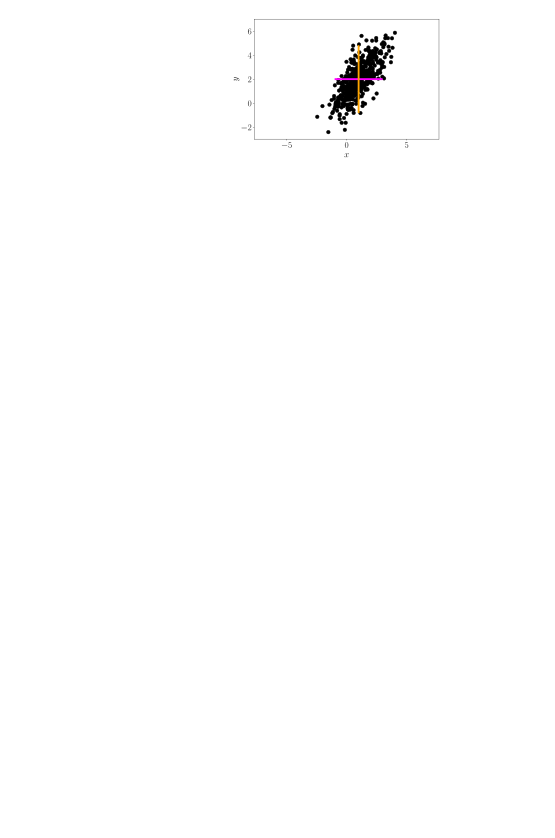
\includegraphics[keepaspectratio]{covarianza2}} 
  \caption{Due dataset bidimensionali con medie e varianze uguali (linee colorate), ma aventi covarianze diverse. Fonte~\cite{deisenrothMML2020}.}
\label{fig:bgvfcd}
\end{figure}


\subsubsection{Proprietà notevoli di media e varianza}

Siano $a, b \in \mathbb{R}$ e $\mathbf{X}, \mathbf{Y}$ due vettori aleatori. Sussistono i seguenti risultati:
\begin{align}
    \mathbb{E}[a\mathbf{X}+b\mathbf{Y}]   & = a\mathbb{E}[\mathbf{X}]+b\mathbb{E}[\mathbf{Y}] \qquad \text{Linearità della media} \label{eq:prop_media1}\\
    \mathbb{E}[a\mathbf{X}+b]   & = a\mathbb{E}[\mathbf{X}]+b \label{eq:prop_media2}\\
    \mathbb{V}ar[a\mathbf{X}+b] & = a^2\mathbb{V}ar[\mathbf{X}] \label{eq:prop_varianza1} \\
    \mathbb{V}ar[a\mathbf{X}+b\mathbf{Y}] & = a^2\mathbb{V}ar[\mathbf{X}] + b^2\mathbb{V}ar[\mathbf{Y}]+2ab\text{Cov}[\mathbf{X},\mathbf{Y}]\label{eq:prop_varianza2}
\end{align}


\subsection{Indipendenza statistica}


\begin{Mybox}
    \begin{definizione}[Indipendenza statistica]
       Due vettori aleatori $\mathbf{X},\mathbf{Y}$ sono \emph{statisticamente indipendenti} se e solo se
    \begin{equation}
        p(\mathbf{x},\mathbf{y})=p(\mathbf{x})p(\mathbf{y})\label{eq:indipendenza}
    \end{equation}
    \end{definizione}
\end{Mybox}


\noindent Intuitivamente, due vettori aleatori $\mathbf{X}$ e $\mathbf{Y}$ sono indipendenti se la 
conoscenza dei valori assunti da uno dei due non dà nessuna informazione sui valori assunti dall'altro. 



Qualora i vettori $\mathbf{X}$ e $\mathbf{Y}$ siano statisticamente indipendenti, risulta che:
\begin{align}
    p(\mathbf{y}| \mathbf{x}) & = p(\mathbf{y}) \\
    p(\mathbf{x}| \mathbf{y}) & = p(\mathbf{x}) \\
    \mathbb{V}ar[\mathbf{X}+\mathbf{Y}] & = \mathbb{V}ar[\mathbf{X}]+\mathbb{V}ar[\mathbf{Y}] \\
    \text{Cov}[\mathbf{X},\mathbf{Y}]   & = \bm{0}
\end{align}


\subsection{Distribuzione gaussiana}

\subsubsection{Variabile aleatoria gaussiana}

\begin{Mybox}
    \begin{definizione}
     Una variabile aleatoria continua $X$ dicesi \emph{gaussiana}, o \emph{normale}, se è descritta dalla seguente \emph{pdf}:
    \begin{equation}
        p(x)=\frac{1}{\sqrt{2 \pi \sigma^2}} \exp \Biggl(-\frac{(x-\mu)^2}{2 \sigma^2}\Biggr)
    \end{equation}    
    \end{definizione}
\end{Mybox}


\noindent Sinteticamente si scrive 
\[
    X \sim \mathcal{N}(\mu, \sigma^2) 
\]
per evidenziare come la \emph{pdf} di una \emph{v.a}.\ gaussiana sia completamente determinata qualora vengano assegnati i due parametri seguenti: 
\begin{itemize}
    \item $\mu=\mathbb{E}[X]\in \mathbb{R}$, la \emph{media statistica} della \emph{v.a}.\ $X$.
    \item $\sigma^2=\mathbb{V}ar[X]$, la \emph{varianza} della \emph{v.a}.\ $X$.
\end{itemize} 

\begin{figure}
    \centering
    \subfloat[][\emph{pdf} di una variabile aleatoria gaussiana standard, $X \sim \mathcal{N}(0, 1)$.]
   {\includegraphics[keepaspectratio, scale=0.38]{normal1D1}} \quad
    \subfloat[][\emph{pdf} di variabili gaussiane con $\mu=2$ e $\sigma^2=4,1,0.25$]
   {\includegraphics[keepaspectratio, scale=0.38]{normal1D2}} 
  \caption{Distribuzioni gaussiane unidimensionali}
\label{fig:normali1D}
\end{figure}

\smallskip 

\noindent Si noti (Figura~\ref{fig:normali1D}) la peculiare forma, tipica di una “campana”, esibita dalla \emph{pdf} di una gaussiana (\emph{bell-shaped pdf}). 
Dalla Figura~\ref{fig:normali1D} è possibile desumere il significato dei due suddetti parametri:
\begin{itemize}
    \item $\mu$ è un \emph{fattore di posizione} che costituisce il centro di simmetria della densità di probabilità.
    Modifiche apportate a tale parametro si riflettono in traslazioni orizzontali rigide della \emph{pdf}. 
    \item $\sigma^2$ è un \emph{fattore di scala} che regola la larghezza della campana attorno alla media $\mu$: all'aumentare di $\sigma^2$ 
    la campana si allarga e diventa più schiacciata (per preservare l'unitarietà dell'area sottesa), mentre 
    al diminuire di $\sigma^2$ corrisponde una campana più stretta e alta (Figura~\ref{fig:normali1D}).
\end{itemize} 



%---------------------------------------------------------------------------------

\subsubsection{Vettore aleatorio gaussiano}

\begin{figure}
    \centering
    \includegraphics[keepaspectratio, scale=0.55]{multivariate_normal}
    \caption{Distribuzione gaussiana bidimensionale}
\end{figure}


\begin{Mybox}
    \begin{definizione}
        Un vettore aleatorio $\mathbf{X}=[X_1,\dots,X_N]^T \in \mathbb{R}^N$ dicesi \emph{gaussiano}, o \emph{normale}, qualora abbia la seguente \emph{pdf}:
        \begin{equation}
               p(\mathbf{x})=\frac{1}{(2\pi)^{N/2}\lvert  \mathbf{\Sigma} \rvert^{1/2} }\exp \biggl(-\frac{1}{2}(\mathbf{x}-\bm{\mu})^{T} \mathbf{\Sigma}^{-1}(\mathbf{x}-\bm{\mu})\biggr)
        \end{equation}
        dove $\mathbf{x}=[x_1,\dots,x_N]^T \in \mathbb{R}^N$ e $\lvert \mathbf{\Sigma} \rvert = \text{det}(\mathbf{\Sigma})$ è il determinante della matrice $\mathbf{\Sigma}$.    
    \end{definizione}
\end{Mybox}

\noindent Sinteticamente si scrive 
\[
    \mathbf{X} \sim \mathcal{N}(\bm{\mu}, \mathbf{\Sigma}) \quad\text{o}\quad p(\mathbf{x})=\mathcal{N}(\mathbf{x};\bm{\mu}, \mathbf{\Sigma})
\]
per evidenziare come la \emph{pdf} del vettore aleatorio $X$ sia completamente determinata qualora vengano assegnati: 
\begin{itemize}
    \item il \emph{vettore delle medie} $\bm{\mu}=\mathbb{E}[\mathbf{X}]=(\mathbb{E}[X_1],\mathbb{E}[X_2],\dots,\mathbb{E}[X_N])^T$.
    \item la \emph{matrice di covarianza} $\mathbf{\Sigma}= \mathbb{E}[(\mathbf{X}-\bm{\mu})(\mathbf{X}-\bm{\mu})^T]\in \mathbb{R}^{N \times N}$.
\end{itemize} 
\smallskip
\begin{oss}[Combinazione lineare di vettori gaussiani indipendenti]\label{oss:comb_lin_normali}
    Siano $\mathbf{X}\sim\mathcal{N}(\bm{\mu}_{\mathbf{X}}, \bm{\Sigma}_{\mathbf{X}})$ e 
    $\mathbf{Y}\sim\mathcal{N}(\bm{\mu}_{\mathbf{Y}}, \bm{\Sigma}_{\mathbf{Y}})$ due vettori aleatori gaussiani \emph{indipendenti}. Siano, inoltre,
    $\bm{A}$ e $\bm{B}$ due matrici. Sussiste il seguente risultato:
    \begin{equation}
     (\bm{A}\mathbf{X}+\bm{B}\mathbf{Y}) \sim \mathcal{N}(\bm{A}\bm{\mu}_{\mathbf{X}} +\bm{B}\bm{\mu}_{\mathbf{Y}}, \bm{A}\bm{\Sigma}_{\mathbf{X}}\bm{A}^T+\bm{B}\bm{\Sigma}_{\mathbf{Y}}\bm{B}^T) \label{eq:comblingauss}
    \end{equation}
    da cui si evince che la combinazione lineare di vettori aleatori gaussiani indipendenti è ancora un vettore aleatorio gaussiano.
    La~\eqref{eq:comblingauss} declinata al caso in cui le suddette matrici siano degli scalari diventa:
    \begin{equation}
        (a\mathbf{X}+b\mathbf{Y}) \sim \mathcal{N}(a\bm{\mu}_{\mathbf{X}} +b\bm{\mu}_{\mathbf{Y}}, a^2\bm{\Sigma}_{\mathbf{X}}+b^2\bm{\Sigma}_{\mathbf{Y}})\label{eq:comblingauss_scalar}
    \end{equation}
\end{oss}

\subsubsection{Trasformazione affine di una v.a.\ gaussiana}
\label{sssec:Reparametrization_Trick}


\begin{Mybox}
    Una variabile aleatoria gaussiana $X \sim \mathcal{N}(\mu, \sigma^2)$ può essere sempre riguardata come
    una \emph{trasformazione affine} (cascata di cambiamento di scala e traslazione) di una 
    \emph{gaussiana standard} $X_0 \sim \mathcal{N}(0, 1)$
    \begin{equation}
        X = \sigma X_0 + \mu,  \qquad \sigma>0, \, \mu \in \mathbb{R} \label{eq:rep_trick}
    \end{equation}
\end{Mybox}


\subsection{Catena Markoviana}\label{ssec:markov_chain}

Siano $\{\mathbf{X}_i\}_{i\in\mathbb{N}\cup0}$ una sequenza di vettori aleatori aventi tutti lo stesso alfabeto 
$\mathcal{A}_{\mathbf{X}_i}=\mathcal{X}$. 

\begin{Mybox}
\begin{definizione}[Proprietà markoviana]\label{def:markov_property}La sequenza $\{\mathbf{X}_i\}$ è una \emph{catena markoviana} se sussiste la seguente proprietà:
    \begin{equation}
    \begin{split}
        &p(\mathbf{x}_n | \mathbf{x}_{n-1},\dots,\mathbf{x}_0)=
        p(\mathbf{x}_n | \mathbf{x}_{n-1}) \\
        & \forall n\in\mathbb{N},\, \forall (\mathbf{x}_0,\dots,\mathbf{x}_n)\in\mathcal{X}^n \label{eq:markov_property}
    \end{split}
    \end{equation}
\end{definizione}
\end{Mybox}

\begin{oss}[Interpretazione]
Interpretando $n-1$ come l'istante presente, $n-j$ (con $j\geq2$) come il passato e $n$ come futuro,
la proprietà markoviana~\eqref{eq:markov_property} asserisce che, in una catena markoviana, 
il futuro è indipendente dal passato dato il presente~\cite{conteFenomeniAleatori2006}.
\end{oss}
\bigskip
\begin{oss}
Avvalendosi della proprietà markoviana, la distribuzione congiunta di $\mathbf{X}_0,\mathbf{X}_1,\dots,\mathbf{X}_n$ ammette 
la seguente riformulazione:
\begin{align}
p(\mathbf{x}_0,\dots,\mathbf{x}_n) &= p(\mathbf{x}_n|\mathbf{x}_{n-1},\dots,\mathbf{x}_0)\,p(\mathbf{x}_{n-1}|\mathbf{x}_{n-2},\dots,\mathbf{x}_0)\dots \label{eq:chain1}\\
                                   &\dots
                                   p(\mathbf{x}_1|\mathbf{x}_0)\,p(\mathbf{x}_0) \label{eq:chain2}\\
                                   &=p(\mathbf{x}_n|\mathbf{x}_{n-1})\,p(\mathbf{x}_{n-1}|\mathbf{x}_{n-2})\dots p(\mathbf{x}_1|\mathbf{x}_0)\,p(\mathbf{x}_0)\label{eq:chain3} \\
                                   &=p(\mathbf{x}_0) \prod_{j=1}^n p(\mathbf{x}_j|\mathbf{x}_{j-1})
\end{align}
dove
\begin{itemize}
    \item nella~\eqref{eq:chain1} si è ricorsi alla \emph{chain rule}~\eqref{eq:chain_rule}.
    \item nel passaggio~\eqref{eq:chain2} alla~\eqref{eq:chain3} si è sfruttata la proprietà markoviana~\eqref{eq:markov_property}.
\end{itemize}
\end{oss}



\section{Problema della stima dei parametri}\label{sec:statistica}

\subsection{Modellazione parametrica}

In statistica, un modello parametrico è una famiglia di distribuzioni $p_{\bm{\theta}}(\mathbf{x})$ descritta 
da un numero finito di \emph{parametri} $\bm{\theta} \in \Theta \subseteq \mathbb{R}^k$, con $\Theta$ detto \emph{spazio dei parametri}.


\subsection{Funzione di verosimiglianza}\label{ssec:verosimiglianza}

Sia $\mathbf{X}$ un vettore aleatorio e $\mathbf{x} \in \mathbb{R}^N$ una sua possibile realizzazione.

\begin{Mybox}
    \begin{definizione}
        Si definisce funzione di verosimiglianza (\emph{likelihood}) la funzione:
        \begin{equation}
        \bm{\theta_i} \in \Theta \longmapsto \mathcal{L}_{\mathbf{x}}(\bm{\theta_i} )= p(\mathbf{x} \mid \bm{\theta}=\bm{\theta_i}) = p_{\bm{\theta_i}}(\mathbf{x})\label{eq:likelihood}
        \end{equation}   
    \end{definizione}
\end{Mybox}

\smallskip
\begin{oss}
Si potrebbe essere erroneamente indotti a ritenere che $\bm{\theta}$, dal momento che si trova a destra del 
condizionamento in $p(\mathbf{x} \mid \bm{\theta}=\bm{\theta_i})$~\eqref{eq:likelihood}, debba essere considerato 
come osservato e fissato: tale interpretazione è errata.
Come suggerisce la notazione, $\mathcal{L}_{\mathbf{x}}(\bm{\theta})$ è una funzione del parametro $\bm{\theta}$, che varia, mentre il dato 
$\mathbf{x}$ è fissato. Inoltre la funzione di verosimiglianza~\eqref{eq:likelihood} non è una distribuzione di probabilità in $\bm{\theta}$.
\end{oss}
\begin{oss}
Allorché risulti chiaro dal contesto, si scrive semplicemente $\mathcal{L}(\bm{\theta})$, 
omettendo il pedice $\mathbf{x}$ che si riferisce ai dati osservati. 
\end{oss}

\begin{oss}[Interpretazione]
La distribuzione $p(\mathbf{x} \mid \bm{\theta}=\bm{\theta_i})$ modella l'incertezza dei 
dati $\mathbf{x}$ per una certa istanza $\bm{\theta_i}$ del parametro $\bm{\theta}$. Dunque, avvalendosi della 
funzione di verosimiglianza, per dei dati fissati $\mathbf{x}$, è possibile capire, al variare del parametro $\bm{\theta}$, qual'è 
l'istanza del parametro che ha generato i dati con maggiore probabilità.
In un'ottica complementare, riguardando i dati come fissati (poiché osservati), e variando il parametro $\bm{\theta}$, la funzione 
di verosimiglianza $\mathcal{L}(\bm{\theta})$ misura quanto è probabile una particolare scelta di $\bm{\theta}$ per le osservazioni $\mathbf{x}$~\cite{deisenrothMML2020}.
\end{oss}

\bigskip
\noindent Se si dispone di un dataset $\mathcal{X}=\{\mathbf{x}_1,\dots,\mathbf{x}_M\}$ di osservazioni tra loro 
indipendenti allora, in virtù della~\eqref{eq:indipendenza}, la funzione di verosimiglianza è:
\begin{equation}
    \mathcal{L}_{\mathcal{X}}(\bm{\theta})=p(\mathcal{X}|\bm{\theta})=p_{\bm{\theta}}(\mathbf{x}_1,\dots,\mathbf{x}_M)=\prod_{\mathbf{x} \in \mathcal{X}} p_{\bm{\theta}}(\mathbf{x}) \label{eq:datasetlikelihood}
\end{equation}


\noindent In letteratura si considera il \emph{logaritmo} della funzione di verosimiglianza cambiato di segno\footnote{il cambiamento di segno è imputabile alla convenzione vigente nella letteratura sull'ottimizzazione numerica, 
in cui si predilige lo studio della minimizzazione di funzioni.} (\emph{negative log-likelihood}):
\begin{equation}
   {\ell}_{\mathbf{x}}(\bm{\theta})=-\log(\mathcal{L}_{\mathbf{x}}(\bm{\theta}))=-\log(p_{\bm{\theta}}(\mathbf{x}))\label{eq:nll}
\end{equation}

\noindent Riformulando la~\eqref{eq:datasetlikelihood} con il logaritmo, risulta che:
\begin{equation}
    {\ell}_{\mathcal{X}}(\bm{\theta})=-\log\bigl(\mathcal{L}_{\mathcal{X}}(\bm{\theta})\bigr)=-\log\Bigl(\prod_{\mathbf{x} \in \mathbf{\mathcal{X}}} p_{\bm{\theta}}(\mathbf{x})\Bigr)=
    \sum_{\mathbf{x} \in \mathbf{\mathcal{X}}}-\log p_{\bm{\theta}}(\mathbf{x}) \label{eq:loglikelihood}
\end{equation}






\subsection{Metodo della massima verosimiglianza}
\label{appendix:MLE}

Nel \emph{metodo della massima verosimiglianza} (MLE) si massimizza la 
funzione di verosimiglianza per trovare un modello che ben si adatti ai dati di interesse:

\begin{equation}
\hat{\bm{\theta}}=\operatorname{argmax}_{\bm{\theta} \in \Theta} \mathcal{L}_{\mathbf{x}}(\bm{\theta}) \label{eq:MLE}
\end{equation}

\noindent Poiché le reti neurali \emph{minimizzano} una funzione di costo, la~\eqref{eq:MLE} può essere riformulata minimizzando la \emph{negative log-likelihood}:
\begin{equation}
\hat{\bm{\theta}}=\operatorname{argmin}_{\bm{\theta}}\bigl({\ell}_{\mathbf{x}}(\bm{\theta})\bigr)=\operatorname{argmin}_{\bm{\theta}}\bigl(-\log p_{\bm{\theta}}(\mathbf{x})\bigr)\label{eq:log_MLE}
\end{equation}
Il minimizzare la \emph{negative log-likelihood} ha un duplice beneficio~\cite{deisenrothMML2020}:
\begin{itemize}
\item il prodotto delle $M$ probabilità nella~\eqref{eq:datasetlikelihood} ($M$ è la cardinalità del dataset) è soggetto a problemi di \emph{underflow} numerico, 
poiché non si possono rappresentare accuratamente numeri molto piccoli come $10^{-256}$. Il logaritmo 
ovvia a tale problema trasformando i prodotti in somme.
\item trasformando i prodotti in somme mediante l'uso del logaritmo, 
il gradiente dei termini nella~\eqref{eq:loglikelihood} è la somma dei gradienti dei singoli addendi. 
In tal modo si evita di ricorrere all'applicazione reiterata della regola del prodotto per calcolare 
il gradiente del prodotto di $M$ termini.
\end{itemize}

\noindent In questa trattazione si investigano i modelli generativi che si avvalgono del metodo di massima verosimiglianza,
dove i parametri $\bm{\theta}$ sono i pesi delle reti neurali del modello.
L'obiettivo è quello di trovare i valori dei suddetti parametri che massimizzano la verosimiglianza 
(o equivalentemente, minimizzano la \emph{negative log-likelihood}) di osservare i dati nel dataset.
Tuttavia, per problemi ad alta dimensionalità dei dati coinvolti, non è possibile, generalmente, calcolare direttamente $p_{\bm{\theta}}(\mathbf{x})$ 
che risulta intrattabile (si veda~\eqref{eq:intractable_likelihood}).


\chapter{Derivazione funzione di costo DDPM}\label{appendix:details_loss}


\begin{figure}
    \centering
    \includegraphics[keepaspectratio, scale=0.5]{VAE_vs_DIff.pdf}
    \caption{VAE e modello di diffusione a confronto. Fonte~\cite{nain2022}.}
    \label{fig:VAE_vs_Diff}
\end{figure}

Riguardando l'immagine $\mathbf{x}_0$ come un dato osservabile e $\mathbf{x}_1,\dots,\mathbf{x}_T$ come variabili \emph{latenti}, 
si ravvisa un'affinità con l'autoencoder variazionale (VAE) (Figura~\ref{fig:VAE_vs_Diff}).

\medskip

\noindent Similitudini:
\begin{itemize}
\item il processo di diffusione in avanti può essere riguardato come l'equivalente dell'encoder di un VAE, che converte 
i dati osservabili in variabili latenti.
\item il processo di diffusione inversa può essere riguardato come l'equivalente del decoder di un VAE, che, partendo dalle 
variabili latenti, fornisce in uscita i dati.
\end{itemize}

\noindent Differenze:
\begin{itemize}
    \item l'encoder e il decoder di un VAE sono due reti neurali che possono essere addestrate congiuntamente, 
    laddove il processo di diffusione in avanti in un DDPM è \emph{fisso} 
    (i.e non annovera parametri che possono essere appresi addestrando un'opportuna rete neurale).
    Soltanto il processo di diffusione inversa si avvale di una rete neurale.
\end{itemize}
Nel paper originale sui VAE (Kingma e Welling~\cite{kingmaVAE2022}), dette $\mathbf{x}$ una variabile osservabile e $\mathbf{z}$ una variabile latente, 
si perviene al seguente risultato:
\begin{equation}
\log p_{\bm{\theta}}(\mathbf{x})\geq \underbrace{\mathbb{E}_{q_{\bm{\phi}}(\mathbf{z}|\mathbf{x})}[\log p_{\bm{\theta}}(\mathbf{x}|\mathbf{z})]
-D_{KL}\bigl(q_{\bm{\phi}}(\mathbf{z}|\mathbf{x})\,\|\,p_{\bm{\theta}}(\mathbf{z})\bigr)}_{\text{Lower Bound Variazionale (ELBO)}} \label{eq:VAE_ELBO}
\end{equation}
Declinando la~\eqref{eq:VAE_ELBO} al contesto dei modelli di diffusione, con $\mathbf{x}_0$ e $\mathbf{x}_{1:T}$ che assurgono rispettivamente a 
dato osservabile e variabili latenti, si ha che~\cite{nain2022}:
\begin{align}
    \log p_{\bm{\theta}}(\mathbf{x})
    &\geq \mathbb{E}_{q(\mathbf{x}_{1:T}|\mathbf{x}_0)}[\log p_{\bm{\theta}}(\mathbf{x}_0|\mathbf{x}_{1:T})]\,-\,
    \mathcolor{blue}{D_{KL}\bigl(q(\mathbf{x}_{1:T}|\mathbf{x}_0)\,\|\,p_{\bm{\theta}}(\mathbf{x}_{1:T})\bigr)} \label{eq:elbo1}\\
    &= \mathbb{E}_{q(\mathbf{x}_{1:T}|\mathbf{x}_0)}[\log p_{\bm{\theta}}(\mathbf{x}_0|\mathbf{x}_{1:T})]\,-
    \,\mathcolor{blue}{\mathbb{E}_{q(\mathbf{x}_{1:T}|\mathbf{x}_0)}\biggl[\log\frac{q(\mathbf{x}_{1:T}|\mathbf{x}_0)}{p_{\bm{\theta}}(\mathbf{x}_{1:T})}\biggr]}\label{eq:elbo2}\\
    &= \mathbb{E}_q[\log p_{\bm{\theta}}(\mathbf{x}_0|\mathbf{x}_{1:T})]\,-\,\mathbb{E}_q\biggl[\log\frac{q(\mathbf{x}_{1:T}|\mathbf{x}_0)}{p_{\bm{\theta}}(\mathbf{x}_{1:T})}\biggr]\label{eq:elbo3}\\
    &=\mathbb{E}_q\biggl[\log p_{\bm{\theta}}(\mathbf{x}_0|\mathbf{x}_{1:T})\,-\,\log\frac{q(\mathbf{x}_{1:T}|\mathbf{x}_0)}{p_{\bm{\theta}}(\mathbf{x}_{1:T})}\biggr]\label{eq:elbo4}\\
    &= \mathbb{E}_q\biggl[\log p_{\bm{\theta}}(\mathbf{x}_0|\mathbf{x}_{1:T})\,+\,\log\frac{p_{\bm{\theta}}(\mathbf{x}_{1:T})}{q(\mathbf{x}_{1:T}|\mathbf{x}_0)}\biggr]\\
    &=\mathbb{E}_q\biggl[\log\frac{p_{\bm{\theta}}(\mathbf{x}_0|\mathbf{x}_{1:T})\,p_{\bm{\theta}}(\mathbf{x}_{1:T})}{q(\mathbf{x}_{1:T}|\mathbf{x}_0)}\biggr]\\
    &= \mathbb{E}_q\biggl[\log\frac{p_{\bm{\theta}}(\mathbf{x}_{0:T})}{q(\mathbf{x}_{1:T}|\mathbf{x}_0)}\biggr]
\end{align}
dove nel passaggio dalla~\eqref{eq:elbo1} alla~\eqref{eq:elbo2} si è sfruttata la definizione di \emph{divergenza di Kullback-Leibler}, 
dalla~\eqref{eq:elbo3} alla~\eqref{eq:elbo4} ci si è avvalsi della linearità dell'operatore di media statistica,
e infine delle proprietà dei logaritmi.

\medskip
\noindent Pertanto risulta che 
\begin{align}
    \log p_{\bm{\theta}}(\mathbf{x})&\geq\mathbb{E}_q\biggl[\log\frac{p_{\bm{\theta}}(\mathbf{x}_{0:T})}{q(\mathbf{x}_{1:T}|\mathbf{x}_0)}\biggr]\\
   \implies-\log p_{\bm{\theta}}(\mathbf{x})&\leq\mathbb{E}_q\biggl[-\log\frac{p_{\bm{\theta}}(\mathbf{x}_{0:T})}{q(\mathbf{x}_{1:T}|\mathbf{x}_0)}\biggr]\triangleq L_{vlb} 
\end{align}
Sostituendo le definizioni~\eqref{eq:forward_process} e~\eqref{eq:reverse_process} delle distribuzioni $q(\mathbf{x}_{1:T}|\mathbf{x}_0)$ e $p_{\bm{\theta}}(\mathbf{x}_{0:T})$ 
e usando le proprietà dei logaritmi:
\begin{equation}
    \begin{split}
    L_{vlb}&=\mathbb{E}_q\biggl[-\log p(\mathbf{x}_T)
    \mathcolor{Purple3}{-\log\frac{\prod_{t=1}^Tp_{\bm{\theta}}(\mathbf{x}_{t-1}|\mathbf{x}_t)}{\prod_{t=1}^Tq(\mathbf{x}_{t}|\mathbf{x}_{t-1})}}\biggr]\\
    &=\mathbb{E}_q\biggl[-\log p(\mathbf{x}_T)
    \mathcolor{Purple3}{-\log\prod_{t=1}^T\frac{p_{\bm{\theta}}(\mathbf{x}_{t-1}|\mathbf{x}_t)}{q(\mathbf{x}_{t}|\mathbf{x}_{t-1})}}\biggr]
    \end{split}
\end{equation}
Usando la poprietà dei logaritmi per cui il logaritmo di un prodotto è la somma dei logaritmi si ha:
\begin{equation}
    L_{vlb}=\mathbb{E}_q\biggl[-\log p(\mathbf{x}_T)
    \mathcolor{Purple3}{-\sum_{t=2}^T\log\frac{p_{\bm{\theta}}(\mathbf{x}_{t-1}|\mathbf{x}_t)}{q(\mathbf{x}_{t}|\mathbf{x}_{t-1})}
    -\log\frac{p_{\bm{\theta}}(\mathbf{x}_0|\mathbf{x}_1)}{q(\mathbf{x}_1|\mathbf{x}_0)}}\biggr] \label{eq:elbo5}
\end{equation}
Ricorrendo all'assunzione di Markov~\eqref{def:markov_property}, per cui l'ulteriore condizionamento a $\mathbf{x}_0$ è pleonastico, e alla legge di Bayes~\eqref{eq:Bayes}:
\begin{align}
    q(\mathbf{x}_t|\mathbf{x}_{t-1})&=q(\mathbf{x}_t|\mathbf{x}_{t-1},\mathbf{x}_0) \label{eq:markov_assumption}\\
    q(\mathbf{x}_t|\mathbf{x}_{t-1},\mathbf{x}_0)&=q(\mathbf{x}_{t-1}|\mathbf{x}_t,\mathbf{x}_0)\frac{q(\mathbf{x}_t|\mathbf{x}_0)}{q(\mathbf{x}_{t-1}|\mathbf{x}_0)}  \label{eq:bayesq}
\end{align}
\begin{oss}
Il condizionamento rispetto a $\mathbf{x}_0$ è essenziale: $q(\mathbf{x}_{t-1}|\mathbf{x}_t,\mathbf{x}_0)$ ammette un'espressione 
in forma chiusa, laddove $q(\mathbf{x}_{t-1}|\mathbf{x}_t)$ è intrattabile.
\end{oss}
\noindent Sostituendo il combinato disposto della~\eqref{eq:markov_assumption} e della~\eqref{eq:bayesq} nella~\eqref{eq:elbo5}:
\begin{equation}
    \mathbb{E}_q\biggl[-\log p(\mathbf{x}_T)
    \underbrace{-\sum_{t=2}^T\log\biggl(\frac{p_{\bm{\theta}}(\mathbf{x}_{t-1}|\mathbf{x}_t)}{q(\mathbf{x}_{t-1}|\mathbf{x}_t,\mathbf{x}_0)}\cdot 
    \frac{q(\mathbf{x}_{t-1}|\mathbf{x}_0)}{q(\mathbf{x}_t|\mathbf{x}_0)}\biggr)}
    -\log\frac{p_{\bm{\theta}}(\mathbf{x}_0|\mathbf{x}_1)}{q(\mathbf{x}_1|\mathbf{x}_0)}\biggr] \label{eq:intermediate_vlb} 
\end{equation}
Focalizzandosi sulla sommatoria centrale nella~\eqref{eq:intermediate_vlb} si ha che:
\begin{equation}
\begin{split}
    &-\sum_{t=2}^T\log\biggl(\frac{p_{\bm{\theta}}(\mathbf{x}_{t-1}|\mathbf{x}_t)}{q(\mathbf{x}_{t-1}|\mathbf{x}_t,\mathbf{x}_0)}\cdot 
    \frac{q(\mathbf{x}_{t-1}|\mathbf{x}_0)}{q(\mathbf{x}_t|\mathbf{x}_0)}\biggr)\\
    &= -\sum_{t=2}^T\log\frac{p_{\bm{\theta}}(\mathbf{x}_{t-1}|\mathbf{x}_t)}{q(\mathbf{x}_{t-1}|\mathbf{x}_t,\mathbf{x}_0)}
    \mathcolor{Blue3}{-\sum_{t=2}^T\log\frac{q(\mathbf{x}_{t-1}|\mathbf{x}_0)}{q(\mathbf{x}_t|\mathbf{x}_0)}} \label{eq:intermediate_steps}
\end{split}
\end{equation}
Isolando il secondo termine di sommatoria, risulta che:
\begin{equation}
    \begin{split}
    &\mathcolor{Blue3}{-\sum_{t=2}^T\log\frac{q(\mathbf{x}_{t-1}|\mathbf{x}_0)}{q(\mathbf{x}_t|\mathbf{x}_0)}}\\
    &=-\sum_{t=2}^T\log q(\mathbf{x}_{t-1}|\mathbf{x}_0)+\sum_{t=2}^T\log q(\mathbf{x}_t|\mathbf{x}_0) \\
    &=\mathcolor{Purple0}{-\sum_{t=1}^{T-1}\log q(\mathbf{x}_t|\mathbf{x}_0)}+\mathcolor{DeepSkyBlue1}{\sum_{t=2}^T\log q(\mathbf{x}_t|\mathbf{x}_0)}\\
    &=\mathcolor{Purple0}{-\log q(\mathbf{x}_1|\mathbf{x}_0)-\cancel{\sum_{t=2}^{T-1}\log q(\mathbf{x}_t|\mathbf{x}_0)}}+\mathcolor{DeepSkyBlue1}{\cancel{\sum_{t=2}^{T-1}\log q(\mathbf{x}_t|\mathbf{x}_0)}+\log q(\mathbf{x}_T|\mathbf{x}_0)} \\
    &=-\log q(\mathbf{x}_1|\mathbf{x}_0)+\log q(\mathbf{x}_T|\mathbf{x}_0) \label{eq:intermediate_steps2}
\end{split}
\end{equation}
Sostituendo il combinato disposto della~\eqref{eq:intermediate_steps} e della~\eqref{eq:intermediate_steps2} nella~\eqref{eq:intermediate_vlb} si ottiene che:
\begin{equation}
    \begin{split}
    L_{vlb}=\mathbb{E}_q\biggl[
        &\mathcolor{blue}{-\log p(\mathbf{x}_T)}-
           \sum_{t=2}^T\log\frac{p_{\bm{\theta}}(\mathbf{x}_{t-1}|\mathbf{x}_t)}{q(\mathbf{x}_{t-1}|\mathbf{x}_t,\mathbf{x}_0)}\\
        &\mathcolor{red}{-\log q(\mathbf{x}_1|\mathbf{x}_0)}\mathcolor{blue}{+\log q (\mathbf{x}_T|\mathbf{x}_0)}
        \mathcolor{red}{-\log\frac{p_{\bm{\theta}}(\mathbf{x}_0|\mathbf{x}_1)}{q(\mathbf{x}_1|\mathbf{x}_0)}}\biggr]
    \end{split}
\end{equation}
da cui, per le regole dei logaritmi:
\begin{equation}
    L_{vlb}=\mathbb{E}_q\biggl[\mathcolor{blue}{-\log \frac{p(\mathbf{x}_T)}{q(\mathbf{x}_T|\mathbf{x}_0)}}
    -\sum_{t=2}^T\log\frac{p_{\bm{\theta}}(\mathbf{x}_{t-1}|\mathbf{x}_t)}{q(\mathbf{x}_{t-1}|\mathbf{x}_t,\mathbf{x}_0)}
    \mathcolor{red}{-\log p_{\bm{\theta}}(\mathbf{x}_0|\mathbf{x}_1)}\biggr]
\end{equation}
Avvalendosi della definizione di \emph{divergenza di Kullback-Leibler}:
\begin{equation}
    \begin{split}
    D_{KL}\bigl(p_1(x)\,\|\,p_2(x)\bigr)
    &\triangleq\int_{-\infty}^{+\infty} p_1(x)\log\frac{p_1(x)}{p_2(x)}\,dx\\
    &=\mathbb{E}_{x\sim p_1(x)}\biggl[\log\frac{p_1(x)}{p_2(x)}\biggr] \\
    &=  \mathbb{E}_{p_1}\biggl[-\log\frac{p_2(x)}{p_1(x)}\biggr]  \label{eq:kullback-leibler}
    \end{split}
\end{equation}
si perviene, infine, al seguente risultato:
\begin{Mybox2}
\begin{equation}
    \begin{split}
    L_{vlb}= &\underbrace{-\log p_{\bm{\theta}}(\mathbf{x}_0|\mathbf{x}_1)}_{L_0}\\
    +&\sum_{t=2}^T \underbrace{D_{KL}\bigl(q(\mathbf{x}_{t-1}|\mathbf{x}_t,\mathbf{x}_0)\,\|\,p_{\bm{\theta}}(\mathbf{x}_{t-1}|\mathbf{x}_t)\bigr)}_{L_{t-1}}\\
    +&\underbrace{D_{KL}\bigl(q(\mathbf{x}_T|\mathbf{x}_0)\,\|\,p(\mathbf{x}_T)\bigr)}_{L_T}\label{eq:final_lvlb}
\end{split}
\end{equation}
\end{Mybox2}


\section*{Espressione analitica di $L_{t-1}$}\label{sec:detailed_loss_term}
Si dimostra che (Sohl-Dickstein et al.~\cite{sohl-dickstein2015}), sebbene $q(\mathbf{x}_{t-1}|\mathbf{x}_t)$ sia intrattabile, 
condizionando ulteriormente rispetto a $\mathbf{x}_0$ si perviene, 
(si veda~\cite{nain2022}), ad una distribuzione gaussiana, che, in quanto tale, è trattabile:
\begin{equation}
    q(\mathbf{x}_{t-1}|\mathbf{x}_t,\mathbf{x}_0) = \mathcal{N}(\mathbf{x}_{t-1}; \tilde{\bm{\mu}}_{t}(\mathbf{x}_t,\mathbf{x}_0),\tilde{\beta_t} \bm{I}) 
\end{equation}
dove 
\begin{align}
    \tilde{\bm{\mu}}_t(\mathbf{x}_t,\mathbf{x}_0) &=  \frac{\sqrt{\alpha_t}(1-\overline{\alpha}_{t-1})}{1-\overline{\alpha}_t}\mathbf{x}_t+
                                                      \frac{\sqrt{\overline{\alpha}_{t-1}}\beta_t}{1-\overline{\alpha}_t}\mathbf{x}_0 \label{eq:simplify}\\
    \tilde{\beta}_t &= \frac{1-\overline{\alpha}_{t-1}}{1-\overline{\alpha}_t}\beta_t
\end{align}
in cui $\alpha_t$ e $\overline{\alpha}_t$ sono definiti nella~\eqref{eq:alphas} e, dipendendo solo dagli iperparametri $\beta_t$, 
possono essere pre-calcolati.

Quindi $\tilde{\beta}_t$ e $\tilde{\bm{\mu}}_t(\mathbf{x}_t,\mathbf{x}_0)$ della distribuzione~\eqref{eq:true} sono i parametri 
che possono essere approssimati dalla media e varianza della distribuzione~\eqref{eq:approx}:
\begin{align}
    q(\mathbf{x}_{t-1}|\mathbf{x}_t,\mathbf{x}_0) &= \mathcal{N}(\mathbf{x}_{t-1}; \tilde{\bm{\mu}}_{t}(\mathbf{x}_t,\mathbf{x}_0),\tilde{\beta_t} \bm{I})\label{eq:true} \\
    p_{\bm{\theta}}(\mathbf{x}_{t-1}|\mathbf{x}_t)&=\mathcal{N}(\mathbf{x}_{t-1};\bm{\mu}_{\bm{\theta}}(\mathbf{x}_t,t),\bm{\Sigma}_{\bm{\theta}}(\mathbf{x}_t,t))\label{eq:approx}
\end{align}
addestrando un'opportuna rete neurale.

Pertanto, $L_{t-1}=D_{KL}\bigl(q(\mathbf{x}_{t-1}|\mathbf{x}_t,\mathbf{x}_0)\,\|\,p_{\bm{\theta}}(\mathbf{x}_{t-1}|\mathbf{x}_t)\bigr)$ 
risulta essere la divergenza di Kullback-Leibler tra due distribuzioni gaussiane e, in quanto tale, ammette un'espressione in forma chiusa.

\medskip
\noindent Sebbene nella~\eqref{eq:approx} la rete neurale possa apprendere sia la media che la varianza, Ho et al.~\cite{ho2020} hanno rilevato sperimentalmente
che l'apprendimento di quest'ultima degrada la qualità dei campioni prodotti dalla rete neurale a valle dell'addestramento.
Hanno deciso, quindi, di addestrare la rete neurale ad apprendere la sola media $\bm{\mu}_{\bm{\theta}}(\mathbf{x}_t,t)$, 
fissando la varianza $\bm{\Sigma}_{\bm{\theta}}(\mathbf{x}_t,t)=\beta_t\bm{I}$. 

Dunque, nella fase di addestramento la rete neurale deve apprendere la media $\bm{\mu}_{\bm{\theta}}(\mathbf{x}_t,t)$, cosicché 
la distribuzione~\eqref{eq:approx1} approssimi quanto più fedelmente possibile la~\eqref{eq:true1}:
\begin{align}
    q(\mathbf{x}_{t-1}|\mathbf{x}_t,\mathbf{x}_0) &= \mathcal{N}(\mathbf{x}_{t-1}; \tilde{\bm{\mu}}_{t}(\mathbf{x}_t,\mathbf{x}_0),\tilde{\beta_t} \bm{I})\label{eq:true1} \\
    p_{\bm{\theta}}(\mathbf{x}_{t-1}|\mathbf{x}_t)&=\mathcal{N}(\mathbf{x}_{t-1};\bm{\mu}_{\bm{\theta}}(\mathbf{x}_t,t),\beta_t\bm{I})\label{eq:approx1}
\end{align}

\noindent Inoltre, Ho et al.~\cite{ho2020} hanno osservato che, avvalendosi dell'artificio di riparametrizzazione~\eqref{eq:rep_trick} $\mathbf{x}_0$ può essere così riguardato:
\begin{equation}
  \mathbf{x}_0=\frac{1}{\sqrt{\overline{\alpha}}_t}(\mathbf{x}_t-\sqrt{1-\overline{\alpha}_t}\bm{\epsilon}) \label{eq:rep_trick3}
\end{equation}
dove $\bm{\epsilon}\sim\mathcal{N}(\bm{0},\bm{I})$.
Dal combinato disposto della~\eqref{eq:simplify} e della~\eqref{eq:rep_trick3} risulta che 
$\tilde{\bm{\mu}}_t$ dipende solo da $\mathbf{x}_t$:
\begin{equation}
    \tilde{\bm{\mu}}_t(\mathbf{x}_t)=\frac{1}{\sqrt{\alpha_t}}\biggl(\mathbf{x}_t-\frac{1-\alpha_t}{\sqrt{1-\overline{\alpha}_t}}\bm{\epsilon}\biggr) \label{eq:true_mean}
\end{equation}
Quindi in ogni passo della diffusione inversa la rete neurale deve approssimare la media nella~\eqref{eq:true_mean}. 
Tuttavia, poiché $\mathbf{x}_t$ è disponibile come input del generico passo di diffusione inversa e gli $\alpha_t$ sono noti a monte della fase di training,
allora apprendere la suddetta media si traduce nell'apprendere il rumore $\bm{\epsilon}_t$ additivo che è stato aggiunto nel corrispondente passo di diffusione in avanti:
\begin{equation}
    \bm{\mu}_{\bm{\theta}}(\mathbf{x}_t,t)=\frac{1}{\sqrt{\alpha_t}}\biggl(\mathbf{x}_t-\frac{1-\alpha_t}{\sqrt{1-\overline{\alpha}_t}}\bm{\epsilon}_{\bm{\theta}}(\mathbf{x}_t,t)\biggr) \label{eq:learned_mean}
\end{equation}

\noindent Quindi il termine $L_{t-1}$ risulta essere:
\begin{equation}
L_{t-1}=D_{KL}\biggl(\mathcal{N}\Bigl(\mathbf{x}_{t-1}; \tilde{\bm{\mu}}_{t}(\mathbf{x}_t,\mathbf{x}_0),\tilde{\beta_t} \bm{I}\Bigr)\,\big\|\,\mathcal{N}\Bigl(\mathbf{x}_{t-1};\bm{\mu}_{\bm{\theta}}(\mathbf{x}_t,t),\beta_t\bm{I}\Bigr)\biggr)
\label{eq:kl_div_gaussians}
\end{equation}
dove $\bm{\mu}_{\bm{\theta}}(\mathbf{x}_t,t)$ è quella della~\eqref{eq:learned_mean}.

Ma la~\eqref{eq:kl_div_gaussians} è la divergenza di Kullback-Leibler tra due distribuzioni gaussiane e, a valle di alcuni calcoli (si veda~\cite{nain2022}), 
si perviene alla seguente riformulazione per $L_{t-1}$:
\begin{equation}
L_{t-1}=\mathbb{E}_{\mathbf{x}_0,\bm{\epsilon}}\biggl[\underbrace{\frac{(1-\alpha_t)^2}{2\alpha_t\beta_t(1-\overline{\alpha}_t)}}_{\text{termine di scalatura}}\Big\Vert \bm{\epsilon}-
\bm{\epsilon}_{\bm{\theta}}(\underbrace{\sqrt{\overline{\alpha}_t}\mathbf{x}_0+\sqrt{1-\overline{\alpha}_t}\bm{\epsilon}}_{\mathbf{x}_t},t)\Big\Vert^2\biggr] \label{eq:almost_final}
\end{equation}

\noindent Infine Ho et al.~\cite{ho2020} hanno osservato sperimentalmente che, ignorando il termine di scalatura nella~\eqref{eq:almost_final}, 
si ottengono prestazioni migliori a valle dell'addestramento del modello. 

Pertanto, ognuno degli $L_{t-1}$ nella~\eqref{eq:final_lvlb} esibisce la seguente espressione semplificata:
\begin{Mybox2}
\begin{equation}
    L_{t-1}^{\text{simple}}=\Vert \bm{\epsilon}-
    \bm{\epsilon}_{\bm{\theta}}(\underbrace{\sqrt{\overline{\alpha}_t}\mathbf{x}_0+\sqrt{1-\overline{\alpha}_t}\bm{\epsilon}}_{\mathbf{x}_t},t)\Vert^2 +C
\end{equation}
\end{Mybox2}

\smallskip
\noindent dove $C$ è una costante che non dipende da $\bm{\theta}$ e, quindi, può essere ignorata durante l'addestramento.
\chapter{U-Net}\label{appendix:unet}

La U-Net è stata introdotta nel $2015$ (Ronneberger et al.,~\cite{ronnebergerUNet2015}), e costituiva, allora, 
lo stato dell'arte nell'ambito della segmentazione delle immagini biomediche.

Si ribadisce che la scelta di una U-Net, nel paper di Ho et al.~\cite{ho2020}, coniuga l'esigenza che le immagini 
a monte e a valle della rete neurale abbiano le stesse dimensioni, con la peculiarità della U-Net di produrre un'immagine 
con le medesime dimensioni dell'immagine in ingresso.

In Figura~\ref{fig:UNet} è riportato il diagramma della U-Net in uno step del processo di diffusione inversa. In particolare sono mostrate esplicitamente le dimensioni
dell'immagine rumorosa $\mathbf{x}_t$ nel suo percorso attraverso la rete. Essendo un'immagine a colori, matematicamente $\mathbf{x}_t$ è un \emph{tensore}.

\begin{figure}
    \centering
    \includegraphics[keepaspectratio, scale=0.4]{UNET.pdf}
    \caption{Diagramma della U-Net in uno step della diffusione inversa. Fonte~\cite{fosterGenerativeDeepLearning2023}.}
    \label{fig:UNet}
\end{figure}

Come si evince dalla Figura~\ref{fig:UNet}, la U-Net è composta da due metà:
\begin{itemize}
\item la parte di \emph{downsampling} (a sinistra in Figura~\ref{fig:UNet}), dove l'immagine viene 
\emph{compressa spazialmente} ma \emph{espansa a livello di canale} (o profondità).
\item la parte di \emph{upsampling} (a destra in Figura~\ref{fig:UNet}), dove l'immagine viene 
\emph{espansa spazialmente} ma \emph{compressa a livello di canale}.
\end{itemize}

\noindent In Figura~\ref{fig:UNet_details} sono riportati i dettagli dei blocchi “\emph{DownBlock}” e “\emph{UpBlock}” della 
Figura~\ref{fig:UNet}. 

In particolare, relativamente all'esempio in Figura~\ref{fig:UNet}, ognuno dei blocchi “\emph{DownBlock}” nella parte di \emph{downsampling} incrementa 
il numero di canali del tensore rappresentante l'immagine mediante l'impiego di due “blocchi residuali”(\emph{ResidualBlock}), 
applicando anche un layer finale “\emph{AveragePooling2D}” per dimezzare la dimensione dell'immagine (si veda Figura~\ref{fig:UNet_details}).

Nella porzione di \emph{upsampling} della U-Net, ognuno dei blocchi “\emph{UpBlock}” applica preliminarmente un layer “\emph{UpSampling2D}” 
atto a raddoppiare le dimensioni dell'immagine, ricorrendo all'interpolazione bilineare~\cite{fosterGenerativeDeepLearning2023}.
Inoltre ognuno degli “\emph{UpBlock}” diminuisce 
il numero di canali dell'immagine mediante l'impiego di due “\emph{ResidualBlock}”, concatenando, al contempo, 
gli output dei blocchi “\emph{DownBlock}” per il tramite delle cosiddette “connessioni scorciatoia” (\emph{skip connection}), 
peculiari della U-Net~\cite{fosterGenerativeDeepLearning2023}.
\begin{figure}[t!]
    \centering
    \includegraphics[keepaspectratio, scale=0.5]{UNET3.pdf}
    \caption{Dettagli dei blocchi “\emph{DownBlock}” e “\emph{UpBlock}” della U-Net di Figura~\ref{fig:UNet}. Fonte~\cite{fosterGenerativeDeepLearning2023}.}
    \label{fig:UNet_details}
\end{figure}





%-------------------------------------------------------------------------
\backmatter
%-------------------------------------------------------------------------


% Bibliography
\printbibliography[heading=bibintoc]  % Prints bibliography and display bibliography to toc



% N:B IMPORTANT!!!
%\mainmatter gives you normal chapter numbering and arabic page numbering.
%\frontmatter gives you UNNUMBERED chapters (so chapter* is redundant) and roman page numbering.
%\backmatter gives you UNNUMBERED chapters (so chapter* is redundant) and arabic page numbering.

\begingroup 
\titleformat{\chapter}
{\normalfont\Huge\bfseries\centering} %shape
{}% label
{} % sep
{}  

\chapter*{Ringraziamenti}


\thispagestyle{empty}



\shapepar{\heartshape}{\fontfamily{qzc}\fontshape{it}\selectfont{
Il primo pensiero è per mio fratello Lorenzo, al quale esprimo gratitutidine e al contempo ammirazione per 
l'eccezionale forza di spirito mostrata dinanzi alle avversità della vita. 
Sobbarcandosi, come un cireneo, di responsabilità gravose, mi ha consentito di raggiungere la fine di questo percorso.
Ringrazio mia madre Rita che ha trovato dentro di sè la forza di andare avanti, nonostante tutta l'oscurità.
Ringrazio, inoltre, i Professori Alessandro Bria e Daniele Pinchera per le parole di stima proferite 
nei miei confronti a valle dei rispettivi esami che, riecheggiando nella mia mente, mi hanno permesso di andare avanti nei momenti più bui.
Ringrazio mio zio Giuseppe, per credere sempre in me e nelle mie potenzialità.
Ringrazio, infine, tutti i miei amici.}}

\endgroup



\end{document}
%- ---------------------------------------------------------